\chapter{多目标、极小极大与双层优化}
\label{chap:opt-multi-minimax-bilevel}

前面各章都默认一件事：候选之间的好坏由一个实数决定，数小者胜。很多实际任务并不满足这一点。部署一个模型时，我们同时在意推理延迟和预测误差，两个候选可能一个更快、一个更准，谁也不比谁全面更好；训练一个对扰动稳健的模型时，参数的好坏要看对手在允许范围内挑出的最坏扰动；用验证误差挑选正则强度时，每个候选强度都要先经过一次训练才能评价。三种情形中，梯度、投影和对偶这些工具仍然可用，但在动用它们之前必须先回答一个更基本的问题：这里所说的“最优答案”究竟是什么。

本章的学习目标是分别为这三类问题说清答案的含义，再说明怎样计算和检查它。多个指标共存时，要规定怎样比较向量，以及怎样由一种偏好选出具体方案；两组变量方向相反时，要规定谁先选、谁后选，以及怎样核对一对候选已经互为最优响应；一个问题嵌套另一个问题的解时，要规定内层的解怎样选出，以及外层目标怎样随外层变量求导。每一类问题都会遇到同一种危险：算法停下来的点满足某个局部条件，却不一定就是原问题所要的答案。

路线依问题的结构而定。第~\ref{sec:opt-mmb-multiobjective}节从支配关系出发，比较加权和与阈值约束两种把向量目标化为标量的办法，再用梯度的凸组合构造同时改善全部指标的方向。第~\ref{sec:opt-mmb-minimax}节由“先选参数、后选最坏扰动”的次序得到极小极大问题，用鞍点与间隙检验候选，再看梯度下降—上升为什么会绕圈、外梯度法怎样校正。第~\ref{sec:opt-mmb-bilevel}节把内层训练看作外层参数的函数，比较对有限步算法求导和对精确解求导的两种超梯度，并检查内层选解是否保持在同一分支。第~\ref{sec:opt-mmb-results-costs}节把三类问题放在“返回什么、花多少代价”的共同标准下比较。序贯决策、反馈控制和多方博弈中的时间顺序与信息结构，留到卷五相应部分研究，这里只建立静态问题的结构和计算工具。

\section{多目标优化}
\label{sec:opt-mmb-multiobjective}

本节处理多个指标同时要求变小的问题，即\term{多目标优化}（multiobjective optimization）。标量优化中任意两个候选都能比较大小；指标变成向量之后，有些候选之间无法比较，“最优”只能先定义为“没有被全面超过”。这样留下的通常是一整批候选，要从中选出一个，还必须补充一种偏好。本节先建立比较关系与解集，再依次讨论两种表达偏好的方式——加权求和与设置阈值，最后讨论不预先给定偏好、只求同时改善全部指标的局部方法。

本节固定可行域$C\subseteq\mathbb R^d$与$m$个都要最小化的指标$f_1,\dots,f_m:C\to\mathbb R$，记$\bm f=(f_1,\dots,f_m)$。这里的$m$是指标个数，与约束个数无关。

\subsection{支配与Pareto最优}
\label{sec:opt-mmb-pareto}

\paragraph{一个有限候选例}
设我们要从六个候选模型中选一个部署，每个模型有两项指标：推理延迟$f_1$（毫秒）和验证误差$f_2$（百分点），数值是教学用的假设数据：
\begin{equation}
\label{eq:opt-mmb-six-candidates}
\begin{aligned}
&A=(1,5),\quad B=(2,2.5),\quad C=(3.5,2.2),\\
&D=(5,1),\quad E=(4,4),\quad F=(6,1).
\end{aligned}
\end{equation}
图~\ref{fig:opt-mmb-pareto-candidates}把它们画在目标平面上。$E$比$B$慢，误差也比$B$大，无论我们更在乎哪一项，都没有理由选$E$。$A$与$D$的关系则不同：$A$更快，$D$更准，单凭这两组数无法断定谁更好。比较向量时，“全面不差且至少一项更好”是唯一不依赖偏好的判断。

\begin{definition}[支配与Pareto最优]
\label{def:opt-mmb-pareto}
设$\bm u,\bm v\in C$。若$f_i(\bm u)\leq f_i(\bm v)$对所有$i$成立，且至少有一个$i$使不等号严格成立，称$\bm u$\term{支配}（dominate）$\bm v$。不被任何可行点支配的$\bm v\in C$称为\term{Pareto最优}（Pareto optimal）点；若不存在可行点$\bm u$使$f_i(\bm u)<f_i(\bm v)$对所有$i$同时成立，则称$\bm v$为\term{弱Pareto最优}（weakly Pareto optimal）点。
\end{definition}

Pareto最优点组成的集合称为Pareto集合，它位于参数空间$C$中；它在$\bm f$下的像称为\term{Pareto前沿}（Pareto front），位于目标空间$\mathbb R^m$中。Pareto最优一定弱Pareto最优，因为所有指标都严格更小的点当然支配它；反过来不成立，弱Pareto点可以被“一项相同、另一项更好”的点支配。

\begin{figure}[!htbp]
  \centering
  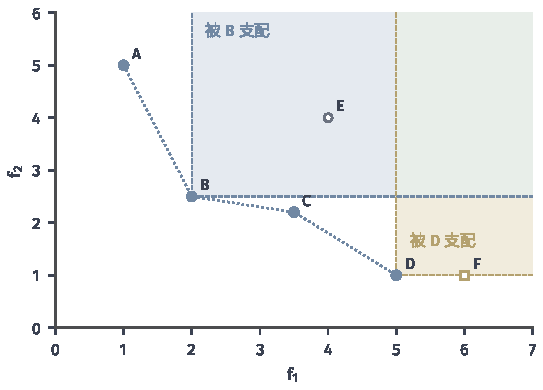
\includegraphics[width=92mm]{figures/03-optimization-evolution-and-signals/01-optimization/matplotlib/c7-pareto-candidates/figure.pdf}
  \caption{式~\eqref{eq:opt-mmb-six-candidates}中六个候选在目标平面上的位置，横轴为延迟$f_1$，纵轴为误差$f_2$。蓝色阴影是被$B$支配的区域，黄色阴影是被$D$支配的区域（重叠部分为绿色）。$E$落在$B$的阴影里；方块$F$落在$D$的阴影边界上，只与$D$误差相同而更慢，所以被支配，却仍是弱Pareto最优。实心点$A,B,C,D$构成Pareto前沿，点线只表示前沿上的顺序。}
  \label{fig:opt-mmb-pareto-candidates}
\end{figure}

\paragraph{有限例中的三类候选}
逐对核对式~\eqref{eq:opt-mmb-six-candidates}即可分类。$E$被$B$（也被$C$）支配；$F$被$D$支配。$A,B,C,D$按延迟递增排列时误差严格递减$5>2.5>2.2>1$，任意两者都是一项更好、一项更差，又不被$E,F$支配，所以都是Pareto最优点。$F$的情形值得注意：要找到两项都严格小于$F=(6,1)$的候选，需要误差小于$1$，而没有候选做到这一点，所以$F$是弱Pareto最优的，尽管它被$D$支配。后面比较各种选择方法时，都以这六个候选为共同对象。

\paragraph{参数空间与目标空间}
连续问题中，Pareto集合与前沿通常是曲线或曲面，二者不在同一个空间。取$C=\mathbb R^2$与
\begin{equation}
\label{eq:opt-mmb-two-quadratics}
f_1(\bm x)=\tfrac12\lVert\bm x-\bm a\rVert_2^2,\qquad f_2(\bm x)=\tfrac12\lVert\bm x-\bm b\rVert_2^2,\qquad \bm a=(1,0),\ \bm b=(-1,0).
\end{equation}
若$x_2\neq0$，把第二个坐标改成零会使两项同时严格减小；若$x_2=0$而$x_1>1$，点$\bm a$使$f_1$减为零、$f_2$也变小；$x_1<-1$时对称。于是只有线段$\{(s,0):-1\leq s\leq1\}$上的点可能是Pareto最优点；在这条线段上，$s$增大使$f_1=(s-1)^2/2$减小而使$f_2=(s+1)^2/2$增大，任意两点互不支配，所以Pareto集合恰是这条线段。图~\ref{fig:opt-mmb-pareto-set-front}左栏画出它，右栏画出它的像：前沿是一段从$(0,2)$到$(2,0)$的曲线，整个平面的像则是曲线右上方的可达集合。图中的点$\bm p=(0,1)$的目标值是$(1,1)$，它被原点支配，原点的目标值是$(1/2,1/2)$。

\begin{figure*}[!htbp]
  \centering
  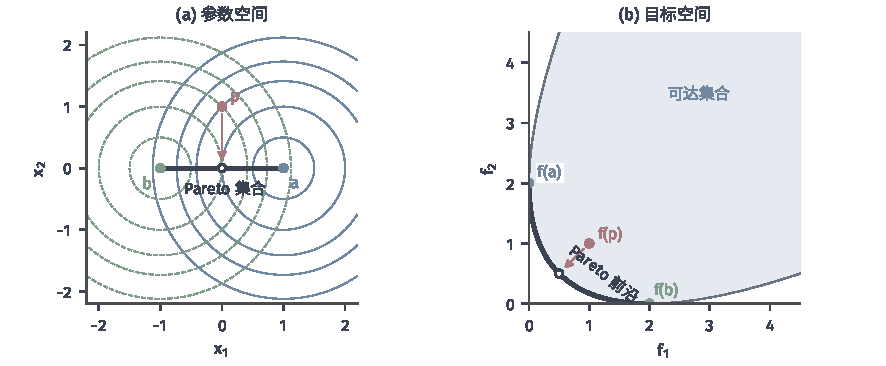
\includegraphics[width=150mm]{figures/03-optimization-evolution-and-signals/01-optimization/matplotlib/c7-pareto-set-front/figure.pdf}
  \caption{同一个双目标问题在两个空间中的样子，目标为式~\eqref{eq:opt-mmb-two-quadratics}。(a)参数平面上，实线圆是$f_1$的等值线，虚线圆是$f_2$的等值线；连接$\bm a,\bm b$的粗线段是Pareto集合。(b)目标平面上，阴影是可达集合$\bm f(\mathbb R^2)=\{(u,v):u+v\geq1+(u-v)^2/4\}$，粗曲线是Pareto前沿$((s-1)^2/2,(s+1)^2/2)$，$-1\leq s\leq1$。红点$\bm p=(0,1)$的像$(1,1)$在可达集合内部，箭头指向支配它的原点之像$(1/2,1/2)$。}
  \label{fig:opt-mmb-pareto-set-front}
\end{figure*}

一个候选不被支配，只说明“没有免费的改进”，并不说明它应当被采用。前沿上的$A$与$D$都是Pareto最优点，却代表截然不同的部署方案。所以多目标问题的输出可以是整个前沿的近似，也可以是按某种偏好选出的一点；下面两小节讨论后者如何确定。

\paragraph{Pareto点何时存在}
Pareto点不会自动存在。取$C=(0,1]$与$f_1(x)=f_2(x)=x$，任意$x$都被更小的$x/2$支配，Pareto集合是空集。缺口出在$C$不是闭集：两个指标共同的下确界$0$不可达。下面的结论用一个严格正权的标量目标把存在性归结为第~\ref{chap:optimization}章的Weierstrass型结论：非空紧集上的连续函数达到最小值。

\begin{theorem}[Pareto点的存在]
\label{thm:opt-mmb-pareto-existence}
设$C$非空紧，$f_1,\dots,f_m$在$C$上连续。则对任意满足$\alpha_i>0$的权重，函数$\sum_{i=1}^m\alpha_if_i$在$C$上达到最小值，且每个最小点都是Pareto最优点。特别地，Pareto集合非空。
\end{theorem}

\begin{proof}
连续函数的正系数线性组合仍连续，非空紧集上的连续函数达到最小值，所以最小点$\bm x^\star$存在。若某个$\bm u\in C$支配$\bm x^\star$，则$\alpha_if_i(\bm u)\leq\alpha_if_i(\bm x^\star)$对所有$i$成立，且对使$f_i(\bm u)<f_i(\bm x^\star)$的那个$i$，由$\alpha_i>0$得到严格不等式。逐项相加得$\sum_i\alpha_if_i(\bm u)<\sum_i\alpha_if_i(\bm x^\star)$，与$\bm x^\star$是最小点矛盾。
\end{proof}

证明中两个条件分工明确：紧性与连续性负责“最小点存在”，权重严格为正负责“最小点不被支配”。有限候选集总是紧的，所以式~\eqref{eq:opt-mmb-six-candidates}的任何正权组合都会选出$A,B,C,D$中的某一个。不过下一小节会看到，“选出的总是Pareto点”并不意味着“每个Pareto点都能被选出”。

\subsection{加权和法}
\label{sec:opt-mmb-weighted-sum}

\paragraph{用权重表达偏好}
最直接的偏好表达是给每个指标一个价格。取权重$\bm\alpha$属于概率单纯形$\Delta_m=\{\bm\alpha\in\mathbb R^m:\alpha_i\geq0,\ \sum_i\alpha_i=1\}$，求解
\begin{equation}
\label{eq:opt-mmb-weighted-sum}
\min_{\bm x\in C}\ \sum_{i=1}^m\alpha_if_i(\bm x).
\end{equation}
这样做的方法称为\term{加权和法}（weighted-sum method），它是把向量目标化为标量的\term{标量化}（scalarization）中最简单的一种。化成标量后，前面各章的方法可以直接使用：目标光滑时用第~\ref{chap:opt-smooth}章的梯度法，带约束时用第~\ref{chap:constrained-optimization}章的方法。

权重的数值本身没有绝对含义，它和指标的单位绑定在一起。若把延迟从毫秒改成秒，$f_1$的数值缩小为原来的千分之一，同一个$\alpha_1$代表的偏好就完全变了。实际使用时常先把每个指标除以一个参考尺度（例如它在候选中的取值范围），再讨论权重。无论权重怎样设定，求解后都应报告每个原始指标，而不是只报告加权值：加权值$2.25$本身无法告诉部署者延迟和误差各是多少。

\paragraph{加权和最小点的Pareto性质}
定理~\ref{thm:opt-mmb-pareto-existence}的证明已经说明正权最小点不被支配。允许某些权重为零时，结论要减弱。

\begin{theorem}[加权和最小点的性质]
\label{thm:opt-mmb-weighted-sum}
设$\bm\alpha\in\Delta_m$，$\bm x^\star$是问题~\eqref{eq:opt-mmb-weighted-sum}的全局最小点。若所有$\alpha_i>0$，则$\bm x^\star$是Pareto最优点；一般情形下，$\bm x^\star$是弱Pareto最优点。
\end{theorem}

\begin{proof}
第一部分的论证与定理~\ref{thm:opt-mmb-pareto-existence}相同。对一般的$\bm\alpha\in\Delta_m$，若有$\bm u\in C$使$f_i(\bm u)<f_i(\bm x^\star)$对所有$i$成立，则由$\alpha_i\geq0$且至少一个$\alpha_i>0$（权重之和为$1$），得$\sum_i\alpha_if_i(\bm u)<\sum_i\alpha_if_i(\bm x^\star)$，矛盾。
\end{proof}

零权确实会带来弱Pareto点。在有限例中取$\bm\alpha=(0,1)$，加权值就是误差$f_2$，$D$与$F$同时达到最小值$1$，而$F$被$D$支配。此时应在加权和的最小点中再剔除被支配者。

\paragraph{加权和只找到凸包上的点}
加权和的几何含义可以在目标平面上看清。固定$\bm\alpha=(\alpha,1-\alpha)$，满足$\alpha u+(1-\alpha)v=c$的点$(u,v)$构成法向为$(\alpha,1-\alpha)$的直线；最小化加权值，就是把这条直线从左下方向右上方平移，直到它第一次碰到可达集合。碰到的位置总在可达集合的“左下凸包”上。前沿若向右上方凹进去一块，任何方向的直线都会先碰到凹陷两侧的点，凹陷内部的点永远不会被选中。

在有限例中计算得
\[
\begin{aligned}
&A:\ 5-4\alpha,\qquad B:\ 2.5-0.5\alpha,\qquad C:\ 2.2+1.3\alpha,\\
&D:\ 1+4\alpha,\qquad E:\ 4,\qquad F:\ 1+5\alpha.
\end{aligned}
\]
$C$不劣于$B$要求$2.2+1.3\alpha\leq2.5-0.5\alpha$，即$\alpha\leq1/6$；$C$不劣于$D$要求$2.2+1.3\alpha\leq1+4\alpha$，即$\alpha\geq4/9$。两个条件不能同时成立，所以无论权重如何，$C$都不会被加权和选中，尽管它是Pareto最优点。几何上，$C$位于连接$B,D$的线段上方：线段在$f_1=3.5$处的高度是$2.5-1.5\times\frac{1.5}{3}=1.75<2.2$。图~\ref{fig:opt-mmb-weighted-sum}把这一现象画在连续前沿和有限候选两个场景中。

\begin{figure*}[!htbp]
  \centering
  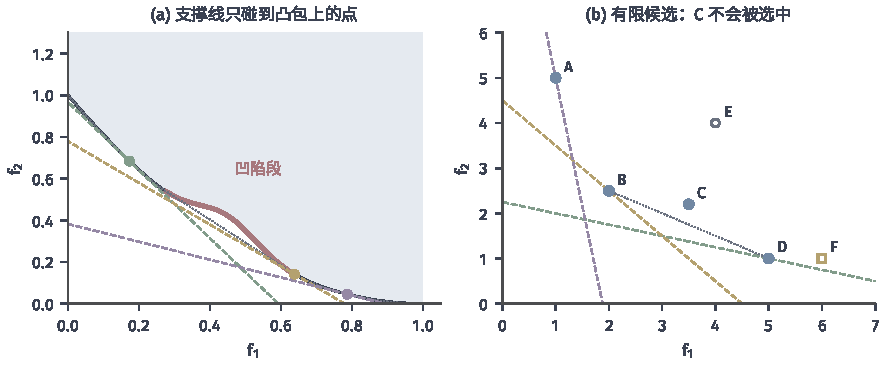
\includegraphics[width=150mm]{figures/03-optimization-evolution-and-signals/01-optimization/matplotlib/c7-weighted-sum/figure.pdf}
  \caption{加权和的支撑线。(a)示意的连续前沿$v=(1-u)^2+0.12\exp(-((u-0.45)/0.12)^2)$，$0\leq u\leq1$（严格递减，每点都是Pareto点），阴影为其右上方的可达区域；三条虚线是$\alpha=0.62,0.5,0.3$时的最低加权等值线，切点分别落在前沿上。点线是前沿的下凸包，红色粗线标出不在凸包上的凹陷段（约$0.27<u<0.63$），没有任何权重能选中其中的点。(b)有限候选中$\alpha=0.85,0.5,0.2$的最低等值线分别经过$A,B,D$；$C$在点线$BD$上方，永远不会被选中。}
  \label{fig:opt-mmb-weighted-sum}
\end{figure*}

如果可达集合向右上方扩张后是凸的（例如$C$凸、各$f_i$凸时），凹陷不会出现。这时可以借助第~\ref{chap:constrained-optimization}章的凸集分离超平面说明：每个弱Pareto点都是某个$\bm\alpha\in\Delta_m$对应的加权和最小点。设$\bar{\bm y}=\bm f(\bar{\bm x})$是弱Pareto点的像，集合$\bm f(C)+\mathbb R^m_{\geq0}$凸，它与开凸集$\{\bm y:y_i<\bar y_i\ \forall i\}$不相交，对差集$\bigl(\bm f(C)+\mathbb R^m_{\geq0}\bigr)-\{\bm y:y_i<\bar y_i\ \forall i\}$这个不含原点的开凸集，用该章的点与闭凸集分离（原点在闭包边界上时，对趋于原点的外点分离再取法向量的极限）得到分离超平面；由于前一集合沿各坐标正方向无界，法向量可取为非负并归一化，这正是所需的权重。非凸问题没有这一保证，所以“扫遍权重即可描出前沿”只在凸情形下可靠。

\paragraph{权重变化与解的跳变}
即使不考虑凹陷，最小点也不必随权重连续移动。有限例中，$\alpha<1/3$时$D$最好，$1/3<\alpha<5/7$时$B$最好，$\alpha>5/7$时$A$最好；$\alpha=1/3$处$B$与$D$并列（加权值都是$7/3$），$\alpha=5/7$处$A$与$B$并列（都是$15/7$）。权重穿过这些临界值时，答案从一个候选跳到另一个，中间的方案没有机会出现。连续问题的前沿若含直线段，同样会在某个权重处出现整段并列的最小点。

\subsection{阈值约束法}
\label{sec:opt-mmb-epsilon-constraint}

\paragraph{把其余指标写成上限}
许多场合的偏好不是价格，而是硬性要求：延迟不能超过某个上限，在此前提下误差越小越好。把这种要求直接写成约束，就得到\term{阈值约束法}（epsilon-constraint method）：保留第$j$个指标作目标，其余指标给出上限$\tau_i$，
\begin{equation}
\label{eq:opt-mmb-epsilon-constraint}
\min_{\bm x\in C}\ f_j(\bm x)\qquad\text{s.t.}\quad f_i(\bm x)\leq\tau_i,\quad i\neq j.
\end{equation}
这是一个普通的约束优化问题，第~\ref{chap:constrained-optimization}章的可行性判断、乘子与求解方法都可以接入。阈值的位置决定约束的状态：阈值过低时问题不可行，应当报告“不存在满足要求的方案”，而不是返回一个违背约束的点；阈值恰好卡住最优解时约束激活，相应乘子度量放宽一单位上限能换来的目标改善；阈值很宽松时约束不起作用，问题退化为只优化$f_j$。

\paragraph{阈值法能到达每个Pareto点}
阈值法与加权和最大的不同在于，它不需要支撑直线，因此能进入凹陷。

\begin{theorem}[阈值约束问题的解]
\label{thm:opt-mmb-epsilon-constraint}
固定$j$与阈值$\tau_i$（$i\neq j$）。
\begin{enumerate}
  \item 问题~\eqref{eq:opt-mmb-epsilon-constraint}的每个全局最小点都是弱Pareto最优点；若全局最小点唯一，它是Pareto最优点。
  \item 反过来，若$\bar{\bm x}$是Pareto最优点，取$\tau_i=f_i(\bar{\bm x})$（$i\neq j$），则$\bar{\bm x}$是问题~\eqref{eq:opt-mmb-epsilon-constraint}的全局最小点。
\end{enumerate}
\end{theorem}

\begin{proof}
(1)设$\hat{\bm x}$是全局最小点。若某个$\bm u\in C$使所有$f_i(\bm u)<f_i(\hat{\bm x})$，则$f_i(\bm u)<f_i(\hat{\bm x})\leq\tau_i$说明$\bm u$可行，而$f_j(\bm u)<f_j(\hat{\bm x})$与最优性矛盾，所以$\hat{\bm x}$弱Pareto最优。若$\hat{\bm x}$是唯一最小点而$\bm u$支配它，则$f_i(\bm u)\leq f_i(\hat{\bm x})\leq\tau_i$说明$\bm u$可行，$f_j(\bm u)\leq f_j(\hat{\bm x})$说明$\bm u$也是最小点，于是$\bm u=\hat{\bm x}$，这与“至少一项严格更小”矛盾。

(2)$\bar{\bm x}$满足$f_i(\bar{\bm x})\leq\tau_i$，是可行点。若某个可行点$\bm u$使$f_j(\bm u)<f_j(\bar{\bm x})$，再由可行性$f_i(\bm u)\leq\tau_i=f_i(\bar{\bm x})$（$i\neq j$），$\bm u$支配$\bar{\bm x}$，与Pareto最优矛盾。
\end{proof}

第二部分不需要任何凸性：只要把阈值设在某个Pareto点的指标值上，那个点就是阈值问题的解。图~\ref{fig:opt-mmb-threshold}左栏中，竖直的阈值线$f_1\leq\tau$从左向右扫过时，选出的点沿整条前沿移动，包括加权和无法到达的凹陷段。代价是：阈值问题的解可能不唯一，此时只能保证弱Pareto性，需要在并列的最小点中再剔除被支配者。

\paragraph{有限例上的预算与价格}
在有限例上以延迟为预算、以误差为目标，计算$\min\{f_2:f_1\leq\tau\}$。$\tau<1$时不可行；$1\leq\tau<2$时只有$A$可行；$2\leq\tau<3.5$时选$B$；$3.5\leq\tau<5$时选$C$；$\tau\geq5$时选$D$，而$\tau\geq6$后$D$与$F$并列，$F$只是弱Pareto点，应剔除。与加权和的结果对照（图~\ref{fig:opt-mmb-threshold}右栏），两种方法在同一个候选集上覆盖的答案不同：预算法能返回$C$，价格法永远不能。两者也都会跳变：预算每跨过一个候选的延迟值，答案就离散地换成另一个候选。

\begin{figure*}[!htbp]
  \centering
  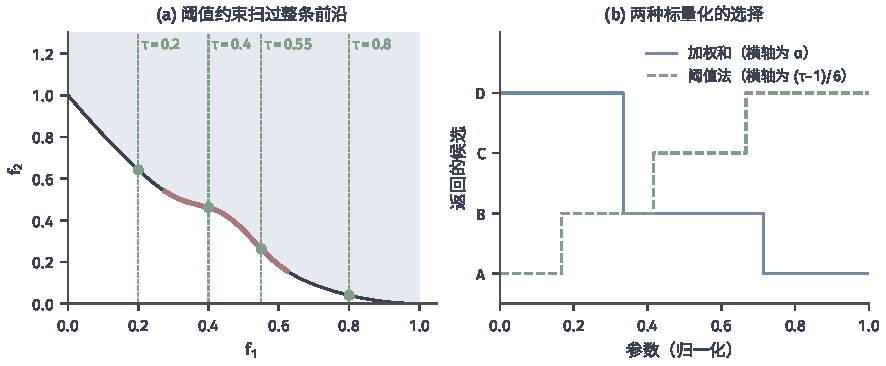
\includegraphics[width=150mm]{figures/03-optimization-evolution-and-signals/01-optimization/matplotlib/c7-threshold/figure.pdf}
  \caption{阈值约束法。(a)与图~\ref{fig:opt-mmb-weighted-sum}(a)相同的前沿，四条竖虚线是延迟上限$\tau=0.2,0.4,0.55,0.8$，圆点是$\min\{f_2:f_1\leq\tau\}$的解；后两个解位于红色凹陷段内，加权和选不到它们。(b)有限例中两种标量化返回的候选：实线是加权和随$\alpha\in[0,1]$的选择，虚线是阈值法随$\tau\in[1,7]$（横轴换算为$(\tau-1)/6$）的选择；并列时按字母顺序取第一个。只有阈值法会返回$C$。}
  \label{fig:opt-mmb-threshold}
\end{figure*}

码率与失真的权衡是同一结构的常见例子：编码方案的码率越低越好，失真也越低越好。给定有限个编码配置时，“码率不超过预算时失真最小”就是阈值问题，“失真加上码率乘以价格最小”就是加权和，二者覆盖的配置可以不同。概率意义下的率失真函数还需要信源分布与信息量的定义，它在\BookChapterRef{chap:information-theory-and-statistical-geometry}{卷四“概率分布的分析与优化”章}中建立，这里只把有限配置当作普通的双指标候选。

\subsection{共同下降方向}
\label{sec:opt-mmb-common-descent}

加权和与阈值法都先把偏好固定下来，再求解一个标量问题。另一种做法是不预设偏好，从当前点出发寻找让所有指标同时下降的方向，直到再也找不到为止。这在指标可微、维数很高（例如多任务学习中共享参数的若干损失）时很自然：每一步只需计算各指标的梯度。

\paragraph{梯度凸包中的最小范数元}
设$C=\mathbb R^d$，各$f_i$在$\bm x$处可微。方向$\bm d$若满足$\langle\nabla f_i(\bm x),\bm d\rangle<0$对所有$i$成立，则沿$\bm d$走足够小的一步，每个指标都严格下降，称它为严格的\term{共同下降方向}（common descent direction）。怎样找到这样的方向？考虑梯度的凸包$\operatorname{conv}\{\nabla f_1(\bm x),\dots,\nabla f_m(\bm x)\}$中离原点最近的点
\begin{equation}
\label{eq:opt-mmb-min-norm}
\bar{\bm g}=\sum_{i=1}^m\alpha_i^\star\nabla f_i(\bm x),\quad
\bm\alpha^\star\in\argmin_{\bm\alpha\in\Delta_m}\ \frac12\Bigl\lVert\sum_{i=1}^m\alpha_i\nabla f_i(\bm x)\Bigr\rVert_2^2.
\end{equation}
权重子问题是单纯形上的凸二次规划，变量个数只有$m$。凸包是非空紧凸集，$\bar{\bm g}$就是原点在它上面的投影，因而唯一（权重$\bm\alpha^\star$未必唯一）。两个指标时子问题有闭式解：记$\bm g_1,\bm g_2$为两个梯度，$\bm g_1\neq\bm g_2$时
\[
\alpha_1^\star=\min\Bigl\{1,\max\Bigl\{0,\frac{\langle\bm g_2,\bm g_2-\bm g_1\rangle}{\lVert\bm g_1-\bm g_2\rVert_2^2}\Bigr\}\Bigr\},
\]
这是对$\lVert\bm g_2+\alpha(\bm g_1-\bm g_2)\rVert_2^2$关于$\alpha$求最小再截断到$[0,1]$的结果。

\begin{lemma}[最小范数元给出共同下降]
\label{lem:opt-mmb-min-norm-descent}
若$\bar{\bm g}\neq\bm 0$，则$\langle\nabla f_i(\bm x),-\bar{\bm g}\rangle\leq-\lVert\bar{\bm g}\rVert_2^2$对所有$i$成立。
\end{lemma}

\begin{proof}
第~\ref{chap:opt-nonsmooth}章建立的投影刻画是：$\bm p$是点$\bm z$在非空闭凸集$K$上的投影，当且仅当$\bm p\in K$且$\langle\bm z-\bm p,\bm v-\bm p\rangle\leq0$对所有$\bm v\in K$成立。取$K$为梯度凸包，$\bm z=\bm 0$，$\bm p=\bar{\bm g}$，$\bm v=\nabla f_i(\bm x)$，得$\langle-\bar{\bm g},\nabla f_i(\bm x)-\bar{\bm g}\rangle\leq0$，整理即为结论。
\end{proof}

\begin{theorem}[一阶共同下降的判据]
\label{thm:opt-mmb-pareto-stationary}
设$C=\mathbb R^d$，各$f_i$在$\bm x$处可微。在$\bm x$处不存在严格的共同下降方向，当且仅当存在$\bm\alpha\in\Delta_m$使$\sum_i\alpha_i\nabla f_i(\bm x)=\bm 0$，即$\bar{\bm g}=\bm 0$。
\end{theorem}

\begin{proof}
若$\sum_i\alpha_i\nabla f_i(\bm x)=\bm 0$而某个$\bm d$使每个$\langle\nabla f_i(\bm x),\bm d\rangle<0$，乘以非负且不全为零的$\alpha_i$后相加得$0=\langle\bm 0,\bm d\rangle<0$，矛盾。反过来，若$\bm 0$不在梯度凸包中，则$\bar{\bm g}\neq\bm 0$，由引理~\ref{lem:opt-mmb-min-norm-descent}，$-\bar{\bm g}$就是严格的共同下降方向。
\end{proof}

满足$\bar{\bm g}=\bm 0$的点常称为Pareto驻点。$m=1$时凸包只有一个梯度，判据退回到$\nabla f_1(\bm x)=\bm 0$。

\paragraph{一个可以手算的例子}
回到式~\eqref{eq:opt-mmb-two-quadratics}的两个二次指标，在$\bm p=(0,1)$处$\nabla f_1(\bm p)=\bm p-\bm a=(-1,1)$，$\nabla f_2(\bm p)=\bm p-\bm b=(1,1)$。闭式解给出$\alpha_1^\star=\langle(1,1),(2,0)\rangle/4=1/2$，$\bar{\bm g}=(0,1)$。两梯度与$-\bar{\bm g}=(0,-1)$的内积都是$-1=-\lVert\bar{\bm g}\rVert_2^2$，与引理一致。沿$-\bar{\bm g}$走步长$1$到达原点，$f_1$与$f_2$都从$1$降到$1/2$；原点处两梯度为$(-1,0)$与$(1,0)$，零向量是它们的平均，不再有共同下降方向。图~\ref{fig:opt-mmb-common-descent}左栏画出了这一步：两条梯度箭头张成的线段上离$\bm p$最近的点决定$\bar{\bm g}$，而所有使两项同时下降的方向组成一个开锥$\{\bm d:d_2<-|d_1|\}$。

\begin{figure*}[!htbp]
  \centering
  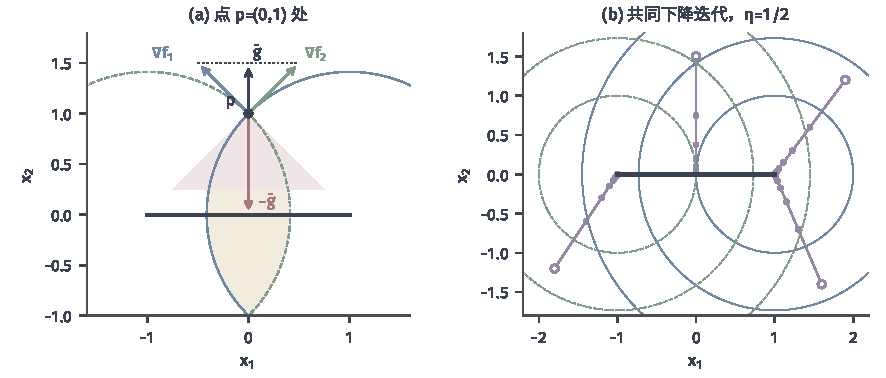
\includegraphics[width=150mm]{figures/03-optimization-evolution-and-signals/01-optimization/matplotlib/c7-common-descent/figure.pdf}
  \caption{共同下降方向，目标为式~\eqref{eq:opt-mmb-two-quadratics}。(a)在$\bm p=(0,1)$处，两条梯度箭头（按$1/2$缩放）之间的点线是梯度凸包，其中最短的向量是$\bar{\bm g}=(0,1)$；红色锥是使两项都严格下降的方向，$-\bar{\bm g}$位于锥的中轴。两段圆弧是过$\bm p$的两条等值线，黄色透镜区域中的点使两项都比在$\bm p$处小。(b)从四个起点出发、步长$\eta=1/2$的共同下降迭代，每条轨迹都停在Pareto集合（粗线段）上，停在哪一点取决于起点。}
  \label{fig:opt-mmb-common-descent}
\end{figure*}

\paragraph{步长与停止}
引理~\ref{lem:opt-mmb-min-norm-descent}只保证方向正确，步长仍要控制。若每个$f_i$的梯度是$L_i$-Lipschitz的（第~\ref{chap:opt-smooth}章的$L$-光滑条件），对每个$i$用二次上界得
\[
f_i(\bm x-\eta\bar{\bm g})\leq f_i(\bm x)-\eta\lVert\bar{\bm g}\rVert_2^2+\frac{L_i\eta^2}{2}\lVert\bar{\bm g}\rVert_2^2,
\]
所以$0<\eta\leq1/\max_iL_i$时每个指标至少下降$\frac{\eta}{2}\lVert\bar{\bm g}\rVert_2^2$。光滑常数未知时，像第~\ref{chap:opt-smooth}章的Armijo回溯那样缩小步长，但接受条件必须对每个指标分别检查。完整的一轮如算法~\ref{alg:opt-mmb-mgda}所示。

\begin{algorithm}[带回溯的共同下降法]
\label{alg:opt-mmb-mgda}
\begin{algorithmic}[1]
\Require 初始点$\bm x^{(0)}$，初始步长$\bar\eta>0$，缩步因子$\rho\in(0,1)$，充分下降常数$c\in(0,1)$，容差$\varepsilon>0$
\Ensure 近似Pareto驻点$\bm x^{(t)}$及各指标值
\For{$t=0,1,2,\dots$}
  \State 计算$m$个梯度$\nabla f_i(\bm x^{(t)})$，解单纯形上的二次规划~\eqref{eq:opt-mmb-min-norm}得$\bar{\bm g}^{(t)}$
  \If{$\lVert\bar{\bm g}^{(t)}\rVert_2\leq\varepsilon$}
    \State \Return $\bm x^{(t)}$与$f_1(\bm x^{(t)}),\dots,f_m(\bm x^{(t)})$
  \EndIf
  \State $\eta\gets\bar\eta$
  \While{存在$i$使$f_i(\bm x^{(t)}-\eta\bar{\bm g}^{(t)})>f_i(\bm x^{(t)})-c\,\eta\lVert\bar{\bm g}^{(t)}\rVert_2^2$}
    \State $\eta\gets\rho\eta$
  \EndWhile
  \State $\bm x^{(t+1)}\gets\bm x^{(t)}-\eta\bar{\bm g}^{(t)}$
\EndFor
\end{algorithmic}
\end{algorithm}

在$L_i$-光滑条件下，上面的二次上界说明$\eta\leq2(1-c)/\max_iL_i$时接受条件对所有$i$成立，所以回溯有限步结束。每轮的代价是$m$次梯度计算、一个$m$维二次规划（形成Gram矩阵$\langle\nabla f_i,\nabla f_k\rangle$需$O(m^2d)$次运算），以及每次试探步上$m$个指标的求值。图~\ref{fig:opt-mmb-common-descent}右栏显示，不同起点停在前沿的不同位置：这一方法只保证“不再能同时改善”，不替我们决定停在哪一种取舍上。

\paragraph{一阶判据的边界}
定理~\ref{thm:opt-mmb-pareto-stationary}是一阶条件，它排除的只是一阶意义下的共同改善，不能代替Pareto最优。取$m=2$、$d=1$、$f_1(x)=f_2(x)=-x^2$，在$x=0$处两梯度都为零，判据成立，而$0$是两个指标共同的极大点，任何$x\neq0$都支配它。再取$f_1(x)=0$、$f_2(x)=x^2$，在$x=1$处$\nabla f_1=0$，取$\bm\alpha=(1,0)$即得零组合，但$x=1$被$x=0$支配。第二个例子中，零组合把全部权重压在一个不随$x$变化的指标上，正对应定理~\ref{thm:opt-mmb-weighted-sum}中零权只保弱Pareto的情形。有约束时，方向还必须保持可行，梯度凸包判据要换成只在可行方向上检查，第~\ref{chap:constrained-optimization}章的可行方向与乘子工具在这里同样需要。

增加凸性后，一阶判据可以加强为全局结论。设各$f_i$在$\mathbb R^d$上凸且可微，$\sum_i\alpha_i\nabla f_i(\bar{\bm x})=\bm 0$，$\bm\alpha\in\Delta_m$。则$\sum_i\alpha_if_i$是凸函数且在$\bar{\bm x}$处梯度为零，由第~\ref{chap:optimization}章的凸函数一阶条件，$\bar{\bm x}$是它的全局最小点；再由定理~\ref{thm:opt-mmb-weighted-sum}，$\bar{\bm x}$是弱Pareto最优点，若所有$\alpha_i>0$则是Pareto最优点。式~\eqref{eq:opt-mmb-two-quadratics}中原点对应$\bm\alpha=(1/2,1/2)$，因此它确实是Pareto最优点，与直接分析一致。

\section{极小极大优化}
\label{sec:opt-mmb-minimax}

多目标问题中，各指标的地位平等，只是需要取舍。另一类问题里，两组变量的利益正好相反：一方要使某个量变小，另一方要使它变大。训练一个对输入扰动稳健的模型时，参数要使损失小，而扰动在允许范围内专挑使损失最大的方向。这时目标值取决于双方的选择次序，本节先把次序和值说清楚，再给出检验一对候选的证书，最后比较两种迭代方法在同一个简单问题上的行为。

本节考虑
\begin{equation}
\label{eq:opt-mmb-minimax}
\min_{\bm x\in X}\ \max_{\bm y\in Y}\ \phi(\bm x,\bm y),
\end{equation}
称为\term{极小极大问题}（minimax problem），其中$X\subseteq\mathbb R^{d}$、$Y\subseteq\mathbb R^{q}$非空，$\phi:X\times Y\to\mathbb R$。$\bm x$是最小化方的变量，$\bm y$是最大化方的变量。

\subsection{响应顺序与最坏值}
\label{sec:opt-mmb-order}

\paragraph{一个猜数游戏}
先看一个一维例子。我们选一个数$x\in\mathbb R$，对手在看到$x$之后从$[-1,1]$中选一个数$y$，我们付出损失$\phi(x,y)=(x-y)^2$。对手看到$x$后会把$y$放到离$x$最远的端点，于是$x$的实际损失是
\[
\bar\phi(x)=\max_{|y|\leq1}(x-y)^2=(|x|+1)^2.
\]
我们应当选$x=0$，最坏损失为$1$。若次序反过来，对手先公布$y$、我们再选$x$，我们只需令$x=y$，损失为零。同一个函数，先选还是后选，得到的值相差$1$。图~\ref{fig:opt-mmb-worst-case}画出了几条$(x-y)^2$及其上包络$\bar\phi$：极小极大问题最小化的是这条上包络，而不是其中任何一条曲线。

\begin{figure}[!htbp]
  \centering
  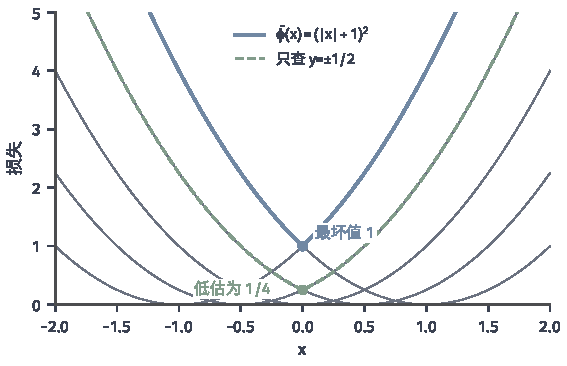
\includegraphics[width=96mm]{figures/03-optimization-evolution-and-signals/01-optimization/matplotlib/c7-worst-case-envelope/figure.pdf}
  \caption{猜数游戏$\phi(x,y)=(x-y)^2$，$y\in[-1,1]$。灰线是$y\in\{0,\pm\frac12,\pm1\}$时的$(x-y)^2$，蓝色粗线是对全部$y\in[-1,1]$取最大的上包络$\bar\phi(x)=(|x|+1)^2$，其最小值$1$在$x=0$处达到。绿色虚线是只检查$y=\pm\frac12$时的包络$(|x|+\frac12)^2$，它把$x=0$的最坏值低估为$1/4$。}
  \label{fig:opt-mmb-worst-case}
\end{figure}

\paragraph{外层值函数}
一般地，问题~\eqref{eq:opt-mmb-minimax}的次序是：外层先选$\bm x$，内层看到$\bm x$后选$\bm y$。外层面对的是值函数
\begin{equation}
\label{eq:opt-mmb-upper-value-function}
\bar\phi(\bm x)=\sup_{\bm y\in Y}\phi(\bm x,\bm y),
\end{equation}
问题~\eqref{eq:opt-mmb-minimax}就是在$X$上最小化$\bar\phi$，其最优值$\overline v=\inf_{\bm x\in X}\bar\phi(\bm x)$称为上值。对称地，定义$\underline\phi(\bm y)=\inf_{\bm x\in X}\phi(\bm x,\bm y)$与下值$\underline v=\sup_{\bm y\in Y}\underline\phi(\bm y)$，它对应内层先选的次序。要让上确界~\eqref{eq:opt-mmb-upper-value-function}确实被某个$\bm y$达到，可以要求$Y$紧且$\phi(\bm x,\cdot)$连续，这正是第~\ref{chap:optimization}章的存在性条件用在内层上。猜数游戏中$Y=[-1,1]$紧，最大值在端点达到。

\begin{lemma}[弱极小极大不等式]
\label{lem:opt-mmb-weak-minimax}
对任意$\phi$与非空的$X,Y$，有$\underline\phi(\bm y)\leq\phi(\bm x,\bm y)\leq\bar\phi(\bm x)$对所有$\bm x\in X,\bm y\in Y$成立，因而$\underline v\leq\overline v$。
\end{lemma}

\begin{proof}
左右两个不等式分别来自下确界与上确界的定义。于是任意$\bm x,\bm y$都满足$\underline\phi(\bm y)\leq\bar\phi(\bm x)$；先对$\bm y$取上确界，再对$\bm x$取下确界即得$\underline v\leq\overline v$。
\end{proof}

不等式说明后选的一方总不吃亏，能看到对方选择的一方至少能做到与先选时一样好。猜数游戏中$\underline v=0<1=\overline v$，等号不成立。

\paragraph{近似内层给出的是下界}
实际计算中，内层的最大化往往只能近似完成。若只在一个子集$Y'\subseteq Y$中搜索，或者内层算法停在某个$\tilde{\bm y}$，所得的$\max_{\bm y\in Y'}\phi(\bm x,\bm y)$或$\phi(\bm x,\tilde{\bm y})$都不超过$\bar\phi(\bm x)$。它们是真实最坏值的下界，而不是外层目标的值。图~\ref{fig:opt-mmb-worst-case}中只检查$y=\pm\frac12$时，$x=0$的最坏损失被报告为$1/4$，而真实值是$1$。若外层据此宣称“最坏损失已降到$1/4$”，结论是错的。要把近似值当作外层目标使用，需要另外控制内层误差，例如内层是凹最大化时用第~\ref{chap:constrained-optimization}章的对偶界给出上界。

允许集合本身也是问题的一部分。把猜数游戏中的$Y$换成$[-\rho,\rho]$，上包络变成$(|x|+\rho)^2$，最坏值变成$\rho^2$。比较两种稳健训练算法之前，必须先确认它们面对的是同一个扰动集合，否则比较的是两个不同的问题。

\subsection{鞍点、间隙与最值交换}
\label{sec:opt-mmb-saddle-gap}

一个候选$\bm x$的好坏由$\bar\phi(\bm x)$决定，而计算$\bar\phi$需要解一个内层最大化。若同时手握一个$\bm y$，能否用一对候选互相印证？答案是比较两个次序下的值。

\begin{definition}[极小极大鞍点]
\label{def:opt-mmb-saddle}
若$(\bm x^\star,\bm y^\star)\in X\times Y$满足
\[
\phi(\bm x^\star,\bm y)\leq\phi(\bm x^\star,\bm y^\star)\leq\phi(\bm x,\bm y^\star)\qquad\text{对所有}\ \bm x\in X,\ \bm y\in Y,
\]
称它为$\phi$在$X\times Y$上的\term{极小极大鞍点}（minimax saddle point）。
\end{definition}

鞍点的含义是双方互为最优响应：固定$\bm y^\star$时，$\bm x^\star$是最小化方的全局最优选择；固定$\bm x^\star$时，$\bm y^\star$是最大化方的全局最优选择。这与多元微积分中由Hessian正负曲率描述的鞍点是两回事。图~\ref{fig:opt-mmb-saddle-surfaces}中两张曲面形状完全相同，都在原点有一个零梯度、Hessian不定的驻点。左图$\phi=x^2-y^2$沿$x$方向向上弯、沿$y$方向向下弯，最小化方$x$与最大化方$y$都在原点取到最优，原点是极小极大鞍点。右图$\phi=y^2-x^2$只是把两个方向的角色交换，此时固定$y=0$，$\phi(x,0)=-x^2$在$x=0$处取最大而非最小，原点不是极小极大鞍点。判断鞍点必须知道哪个变量属于哪一方。

\begin{figure*}[!htbp]
  \centering
  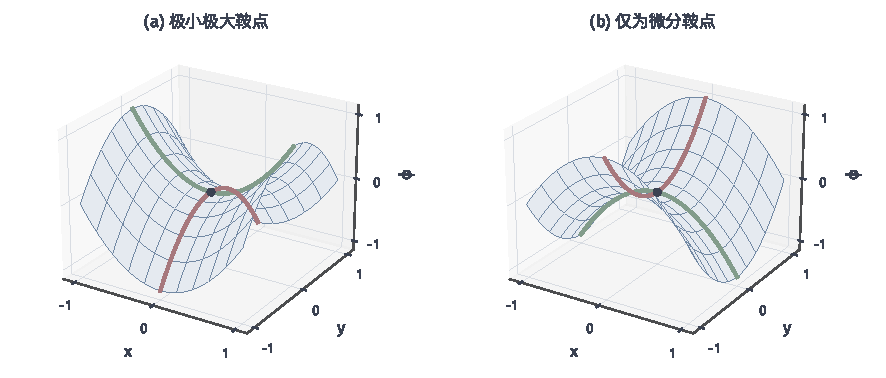
\includegraphics[width=150mm]{figures/03-optimization-evolution-and-signals/01-optimization/matplotlib/c7-saddle-surfaces/figure.pdf}
  \caption{同一形状的马鞍曲面，$x$是最小化方，$y$是最大化方。绿线是$y=0$时沿$x$的截线，红线是$x=0$时沿$y$的截线。(a)$\phi=x^2-y^2$：绿线在原点取最小、红线在原点取最大，原点是极小极大鞍点。(b)$\phi=y^2-x^2$：截线方向反了，原点只是Hessian不定的驻点，最小化方离开原点反而有利。}
  \label{fig:opt-mmb-saddle-surfaces}
\end{figure*}

\paragraph{原始--对偶间隙}
对一对候选$(\bm x,\bm y)$，定义
\begin{equation}
\label{eq:opt-mmb-gap}
\operatorname{gap}(\bm x,\bm y)=\bar\phi(\bm x)-\underline\phi(\bm y),
\end{equation}
称为\term{原始--对偶间隙}（primal--dual gap）。由引理~\ref{lem:opt-mmb-weak-minimax}它总是非负的。

\begin{lemma}[间隙作为证书]
\label{lem:opt-mmb-gap-certificate}
设$\bar\phi(\bm x)$与$\underline\phi(\bm y)$有限。则$\operatorname{gap}(\bm x,\bm y)=0$当且仅当$(\bm x,\bm y)$是极小极大鞍点。此外总有$\bar\phi(\bm x)-\overline v\leq\operatorname{gap}(\bm x,\bm y)$与$\underline v-\underline\phi(\bm y)\leq\operatorname{gap}(\bm x,\bm y)$。
\end{lemma}

\begin{proof}
若$(\bm x,\bm y)$是鞍点，定义中的不等式对所有$\bm x',\bm y'$成立，取上确界与下确界得$\bar\phi(\bm x)\leq\phi(\bm x,\bm y)\leq\underline\phi(\bm y)$，结合非负性得间隙为零。反过来，若$\bar\phi(\bm x)=\underline\phi(\bm y)$，由$\underline\phi(\bm y)\leq\phi(\bm x,\bm y)\leq\bar\phi(\bm x)$知三者相等，于是对所有$\bm x',\bm y'$有$\phi(\bm x,\bm y')\leq\bar\phi(\bm x)=\phi(\bm x,\bm y)=\underline\phi(\bm y)\leq\phi(\bm x',\bm y)$。最后两个不等式由$\underline\phi(\bm y)\leq\underline v\leq\overline v$得到。
\end{proof}

间隙的意义在于它把一个需要“对所有$\bm x',\bm y'$检查”的定义，变成两个最优响应问题的数值：算出$\bar\phi(\bm x)$与$\underline\phi(\bm y)$，相减即可知道$\bm x$离最优上值至多差多少。代价是要能精确求出两侧的最优响应，或至少给出$\bar\phi(\bm x)$的上界与$\underline\phi(\bm y)$的下界。

\paragraph{双线性盒例}
取$X=Y=[-1,1]$，$\phi(x,y)=xy$。固定$x$时$xy$关于$y$线性，最大值在端点，$\bar\phi(x)=|x|$；同理$\underline\phi(y)=-|y|$。于是$\overline v=\underline v=0$，$\operatorname{gap}(x,y)=|x|+|y|$，唯一鞍点是原点。这个例子在后两小节反复使用：它简单到可以手算，却已经足以让最直接的算法失败。

\paragraph{凸凹条件下的最值交换}
猜数游戏中上值严格大于下值，鞍点不存在。什么条件下两个次序给出同一个值？关键是凸凹结构。

\begin{theorem}[紧凸凹条件下的极小极大定理]
\label{thm:opt-mmb-minimax}
设$X,Y$非空、紧、凸，$\phi$在$X\times Y$上连续，对每个$\bm y\in Y$，$\phi(\cdot,\bm y)$在$X$上凸；对每个$\bm x\in X$，$\phi(\bm x,\cdot)$在$Y$上凹。则
\[
\min_{\bm x\in X}\max_{\bm y\in Y}\phi(\bm x,\bm y)=\max_{\bm y\in Y}\min_{\bm x\in X}\phi(\bm x,\bm y),
\]
两侧的最值都能达到，且存在极小极大鞍点。
\end{theorem}

\begin{proof}
由引理~\ref{lem:opt-mmb-weak-minimax}，只需证$\underline v\geq\overline v$。连续函数在紧集上有界，所以$\overline v$有限。任取$c<\overline v$。

第一步，用紧性化为有限个$\bm y$。对每个$\bm x\in X$有$\bar\phi(\bm x)\geq\overline v>c$，故存在$\bm y$使$\phi(\bm x,\bm y)>c$。于是集合$U_{\bm y}=\{\bm x\in X:\phi(\bm x,\bm y)>c\}$覆盖$X$；它们由连续性是$X$中的开集，紧性给出有限个$\bm y_1,\dots,\bm y_k$使每个$\bm x$至少满足一个$\phi(\bm x,\bm y_i)>c$。函数$\bm x\mapsto\max_i\phi(\bm x,\bm y_i)$连续，在紧集$X$上达到最小值，记为$c'$，则$c'>c$。

第二步，用凸性与分离得到权重。令$K=\{\bm z\in\mathbb R^k:\text{存在}\ \bm x\in X\ \text{使}\ z_i\geq\phi(\bm x,\bm y_i)\ \forall i\}$。由$X$凸与每个$\phi(\cdot,\bm y_i)$凸，$K$是凸集。$K$与开凸集$O=\{\bm z:z_i<c'\ \forall i\}$不相交，否则会有$\bm x$使$\max_i\phi(\bm x,\bm y_i)<c'$。为得到分离方向，考虑差集$D=K-O=\{\bm z-\bm w:\bm z\in K,\ \bm w\in O\}$。它是凸集，又因$O$是开集而为开集，且不含原点。第~\ref{chap:constrained-optimization}章由投影证明了点与闭凸集的严格分离；把它用在$D$的闭包上：开凸集的闭包与它有相同的内部，所以原点或者在闭包之外，可以直接严格分离，或者落在闭包的边界上，这时取闭包之外趋于原点的点逐一分离，单位法向量有收敛子列，极限仍是单位向量（与该章强对偶证明中取分离方向极限的做法相同）。两种情形都给出非零$\bm\lambda\in\mathbb R^k$，使$\langle\bm\lambda,\bm z-\bm w\rangle\geq0$，即$\langle\bm\lambda,\bm z\rangle\geq\langle\bm\lambda,\bm w\rangle$对所有$\bm z\in K$、$\bm w\in O$成立。$K$中的点把任一分量增大后仍在$K$中，若某个$\lambda_i<0$，左侧可趋于$-\infty$，矛盾，所以$\bm\lambda\geq\bm 0$，可归一化为$\sum_i\lambda_i=1$。令$\bm w$趋于$(c',\dots,c')$，得$\sum_i\lambda_i\phi(\bm x,\bm y_i)\geq c'$对所有$\bm x\in X$成立。

第三步，用凹性把有限个$\bm y_i$合成一个。令$\bar{\bm y}=\sum_i\lambda_i\bm y_i$，由$Y$凸知$\bar{\bm y}\in Y$；由$\phi(\bm x,\cdot)$凹，$\phi(\bm x,\bar{\bm y})\geq\sum_i\lambda_i\phi(\bm x,\bm y_i)\geq c'$对所有$\bm x$成立。于是$\underline v\geq\underline\phi(\bar{\bm y})\geq c'>c$。由$c<\overline v$的任意性得$\underline v\geq\overline v$。

最后，$\bar\phi$是一族连续函数的上确界，因而下半连续，在紧集$X$上达到最小值；同理$\underline\phi$上半连续，在$Y$上达到最大值。取相应的最优点$\bm x^\star,\bm y^\star$，其间隙为$\overline v-\underline v=0$，由引理~\ref{lem:opt-mmb-gap-certificate}它们构成鞍点。
\end{proof}

证明中每个条件各有职责。紧性与连续性把无穷多个对手选择化为有限个，并保证最值达到；关于$\bm x$的凸性使集合$K$凸，从而能被分离出权重；关于$\bm y$的凹性把“按权重混合几个$\bm y_i$”合成为$Y$中的一个点。猜数游戏缺的正是最后一条：$(x-y)^2$关于$y$是凸的，对手在$y=\pm1$之间的“混合”$\frac12(x+1)^2+\frac12(x-1)^2=x^2+1$不小于$1$，但单点$y=0$只给出$x^2$，混合无法合成为一个纯选择。这一定理是Sion所证更一般结论的特例\cite{sion1958}。

在非凸对抗问题中，例如参数和扰动都经过深度网络的稳健训练，凸凹条件通常不成立，上值与下值可以不同，也无法保证鞍点存在。零梯度也不能代替间隙证书：在$X=Y=[-1,1]$上取$\phi=y^2-x^2$，原点处两个偏梯度都为零，但$\bar\phi(0)=\max_y y^2=1$，$\underline\phi(0)=\min_x(-x^2)=-1$，间隙为$2$。

\subsection{梯度下降—上升}
\label{sec:opt-mmb-gda}

最自然的算法是让双方各按自己的方向走一步：最小化方沿负梯度，最大化方沿正梯度，再各自投影回可行集。设$\phi$在包含$X\times Y$的开集上可微，$X,Y$为非空闭凸集，$\Pi_X,\Pi_Y$是第~\ref{chap:opt-nonsmooth}章的欧氏投影。

\paragraph{同时更新与交替更新}
同时版本中，两个偏梯度都在同一个旧点$(\bm x^{(t)},\bm y^{(t)})$处计算，见算法~\ref{alg:opt-mmb-gda}。交替版本先更新$\bm x$，再在新的$\bm x^{(t+1)}$处计算$\bm y$的梯度：
\[
\begin{aligned}
\bm x^{(t+1)}&=\Pi_X\bigl(\bm x^{(t)}-\eta\nabla_{\bm x}\phi(\bm x^{(t)},\bm y^{(t)})\bigr),\\
\bm y^{(t+1)}&=\Pi_Y\bigl(\bm y^{(t)}+\eta\nabla_{\bm y}\phi(\bm x^{(t+1)},\bm y^{(t)})\bigr).
\end{aligned}
\]
两者的差别只在一个梯度的求值位置，却是不同的迭代，下面会看到它们的轨迹也不同。讨论任何轨迹之前，都要先固定步长、投影规则和更新次序。

\begin{algorithm}[投影同时梯度下降—上升]
\label{alg:opt-mmb-gda}
\begin{algorithmic}[1]
\Require 初始点$\bm x^{(0)}\in X$，$\bm y^{(0)}\in Y$，步长$\eta>0$，迭代次数$T$
\Ensure 迭代点$(\bm x^{(T)},\bm y^{(T)})$，以及可用时的间隙估计
\For{$t=0,1,\dots,T-1$}
  \State 在同一点计算$\bm g_x\gets\nabla_{\bm x}\phi(\bm x^{(t)},\bm y^{(t)})$，$\bm g_y\gets\nabla_{\bm y}\phi(\bm x^{(t)},\bm y^{(t)})$
  \State $\bm x^{(t+1)}\gets\Pi_X(\bm x^{(t)}-\eta\bm g_x)$，$\bm y^{(t+1)}\gets\Pi_Y(\bm y^{(t)}+\eta\bm g_y)$
\EndFor
\end{algorithmic}
\end{algorithm}

\paragraph{双线性问题上的绕圈}
先去掉约束，看$\phi(x,y)=xy$在全平面上的行为。$\nabla_x\phi=y$，$\nabla_y\phi=x$，同时更新为
\[
\begin{pmatrix}x^{(t+1)}\\y^{(t+1)}\end{pmatrix}=\begin{pmatrix}1&-\eta\\ \eta&1\end{pmatrix}\begin{pmatrix}x^{(t)}\\y^{(t)}\end{pmatrix}.
\]
这个矩阵是旋转矩阵乘以$\sqrt{1+\eta^2}$，直接计算得$(x^{(t+1)})^2+(y^{(t+1)})^2=(1+\eta^2)\bigl((x^{(t)})^2+(y^{(t)})^2\bigr)$。每一步都绕鞍点转一个角度并向外放大，任何非零初值都螺旋式地远离鞍点。原因可以从向量场看出：$(-\nabla_x\phi,\nabla_y\phi)=(-y,x)$处处垂直于指向鞍点的方向，沿它走一小段直线，总是落在更大的圆上。

交替版本的矩阵是$\begin{pmatrix}1&-\eta\\ \eta&1-\eta^2\end{pmatrix}$，其行列式为$1$，迹为$2-\eta^2$。当$0<\eta<2$时迹的绝对值小于$2$，两个特征值是模为$1$的一对共轭复数，所以迭代点保持有界，但不趋于鞍点，而是在一条闭曲线附近永远转下去。图~\ref{fig:opt-mmb-gda-bilinear}画出了两种轨迹以及下一小节外梯度法的轨迹。

\begin{figure*}[!htbp]
  \centering
  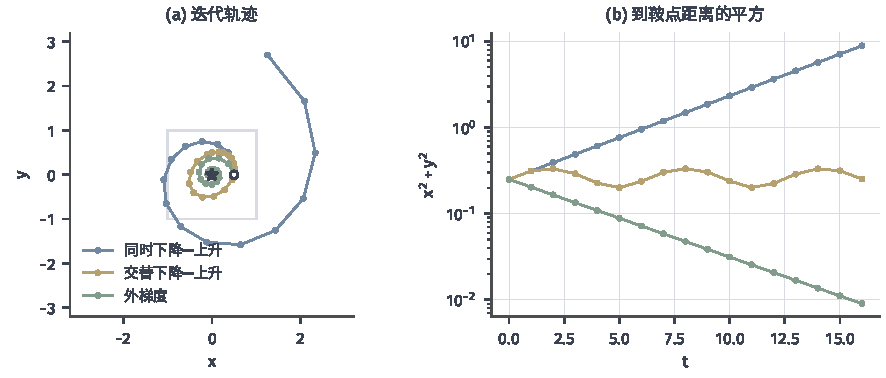
\includegraphics[width=150mm]{figures/03-optimization-evolution-and-signals/01-optimization/matplotlib/c7-gda-bilinear/figure.pdf}
  \caption{双线性目标$\phi(x,y)=xy$上的三种无约束迭代，步长$\eta=1/2$，起点$(1/2,0)$，共16步。(a)轨迹：同时下降—上升（蓝）向外螺旋，交替下降—上升（黄）在闭曲线附近打转，外梯度（绿）向内螺旋；灰框是盒$[-1,1]^2$，星号是鞍点。(b)到鞍点距离的平方（对数坐标）：蓝线每步乘$1+\eta^2=1.25$，绿线每步乘$1-\eta^2+\eta^4=0.8125$，黄线有界振荡。}
  \label{fig:opt-mmb-gda-bilinear}
\end{figure*}

\paragraph{加上投影也不收敛}
有界约束能阻止发散，却不能让迭代停到鞍点。在盒$X=Y=[-1,1]$上取$\eta=1$，从$(1,0)$出发执行算法~\ref{alg:opt-mmb-gda}：
\[
\begin{aligned}
&(1,0)\to(1,1)\to(0,1)\to(-1,1)\to(-1,0)\\
&\quad\to(-1,-1)\to(0,-1)\to(1,-1)\to(1,0).
\end{aligned}
\]
例如第一步$x^{(1)}=\Pi(1-0)=1$，$y^{(1)}=\Pi(0+1)=1$；第二步$x^{(2)}=\Pi(1-1)=0$，$y^{(2)}=\Pi(1+1)=1$。八步之后回到起点，间隙$|x|+|y|$在循环上始终不小于$1$，见图~\ref{fig:opt-mmb-box-cycle}。鞍点存在（定理~\ref{thm:opt-mmb-minimax}的条件全部满足），算法却不收敛：存在性定理回答的是“答案在不在”，不回答“这个算法能否找到它”。

\begin{figure}[!htbp]
  \centering
  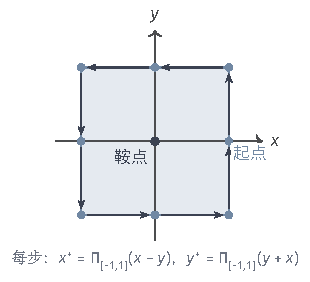
\includegraphics[width=52.5mm]{figures/03-optimization-evolution-and-signals/01-optimization/tikz/c7-box-cycle/figure.pdf}
  \caption{盒约束双线性问题上的投影同时梯度下降—上升，$\phi(x,y)=xy$，$X=Y=[-1,1]$，步长$\eta=1$。从$(1,0)$出发，迭代沿盒的四角与四边中点逆时针循环，周期为$8$；循环上的间隙$|x|+|y|$取$1$或$2$，永不趋于零。}
  \label{fig:opt-mmb-box-cycle}
\end{figure}

这个循环的八个点的平均恰好是原点，那是对称性的巧合。无约束的同时版本中，平均点$\frac1T\sum_{t<T}\bm u^{(t)}$的范数随$T$增大而趋于无穷，因为$\bm u^{(t)}$的范数以$(1+\eta^2)^{t/2}$的速度增长，平均也挽救不了。

\paragraph{用什么判断成功}
极小极大迭代是否成功，要看输出满足的是哪一种关系：可行性（投影后自动满足），间隙~\eqref{eq:opt-mmb-gap}，或者在凸凹且光滑时的投影残差$\lVert\bm u-\Pi_{X\times Y}(\bm u-\eta\bm F(\bm u))\rVert_2/\eta$（$\bm F$见下一小节）。单看某一方的目标是否下降没有意义。双线性例中，点$(0,y)$处$\phi=0$已经等于鞍点值，但它的间隙是$|y|$；最小化方的目标$\bar\phi(x)$可能在一段时间内下降，而最大化方此时正在变差。

\subsection{外梯度法}
\label{sec:opt-mmb-extragradient}

梯度下降—上升的问题在于，它用旧点的方向走一整步，而旋转向量场在一步之内就已经转向。外梯度法先试探性地走一步，看看那里的方向，再回到旧点按试探点的方向走。

\paragraph{两次求值、两次投影}
把双方合成一个变量$\bm u=(\bm x,\bm y)\in K=X\times Y$，令
\begin{equation}
\label{eq:opt-mmb-monotone-field}
\bm F(\bm u)=\bigl(\nabla_{\bm x}\phi(\bm x,\bm y),\ -\nabla_{\bm y}\phi(\bm x,\bm y)\bigr),
\end{equation}
则同时梯度下降—上升就是$\bm u^{(t+1)}=\Pi_K(\bm u^{(t)}-\eta\bm F(\bm u^{(t)}))$。\term{外梯度法}（extragradient method）\cite{korpelevich1976}每轮做两步：
\begin{equation}
\label{eq:opt-mmb-extragradient}
\bar{\bm u}^{(t)}=\Pi_K\bigl(\bm u^{(t)}-\eta\bm F(\bm u^{(t)})\bigr),\qquad
\bm u^{(t+1)}=\Pi_K\bigl(\bm u^{(t)}-\eta\bm F(\bar{\bm u}^{(t)})\bigr).
\end{equation}
第二步的起点仍是旧点$\bm u^{(t)}$，只是方向换成了试探点$\bar{\bm u}^{(t)}$处的方向。这与连续做两次普通梯度步不同：后者的第二步从$\bar{\bm u}^{(t)}$出发。每轮需要两次方向求值（各含一次$\nabla_{\bm x}\phi$与$\nabla_{\bm y}\phi$）和两次投影，返回$\bm u^{(t+1)}$，下面的平均保证则作用于试探点的平均。

\paragraph{双线性例中的校正}
仍取$\phi(x,y)=xy$，$\bm F(x,y)=(y,-x)$。图~\ref{fig:opt-mmb-extragradient-step}取旧点$\bm u=(1.6,0)$与$\eta=1/2$：$\bm F(\bm u)=(0,-1.6)$，试探点$\bar{\bm u}=(1.6,0.8)$；$\bm F(\bar{\bm u})=(0.8,-1.6)$，从旧点出发的校正点为$\bm u^+=(1.6-0.4,\,0+0.8)=(1.2,0.8)$，到鞍点的距离从$1.6$降到$\sqrt{2.08}\approx1.44$。若从试探点再走一次普通步，会到达$(1.2,1.6)$，距离增到$2$。试探点的方向已经“转过了一点”，用它从旧点出发，正好抵消了旋转造成的外漂。

\begin{figure}[!htbp]
  \centering
  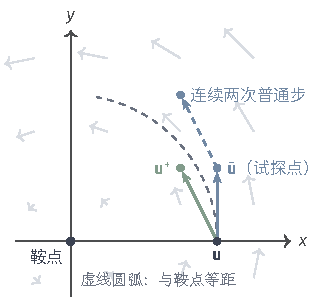
\includegraphics[width=54.0mm]{figures/03-optimization-evolution-and-signals/01-optimization/tikz/c7-extragradient-step/figure.pdf}
  \caption{外梯度法的一步，$\phi(x,y)=xy$，$\eta=1/2$。灰色短箭头是更新方向场$-\bm F=(-y,x)$，绕鞍点旋转。从旧点$\bm u=(1.6,0)$出发，普通步到达试探点$\bar{\bm u}=(1.6,0.8)$，若再走一次普通步（蓝色虚线）会到$(1.2,1.6)$；外梯度从$\bm u$出发、沿$\bar{\bm u}$处的方向走，得到$\bm u^+=(1.2,0.8)$（绿色），落在过$\bm u$的等距圆弧以内。}
  \label{fig:opt-mmb-extragradient-step}
\end{figure}

一般地，无约束时把式~\eqref{eq:opt-mmb-extragradient}代入$\bm F(x,y)=(y,-x)$得
\[
\bm u^{(t+1)}=\begin{pmatrix}1-\eta^2&-\eta\\ \eta&1-\eta^2\end{pmatrix}\bm u^{(t)},\qquad
\lVert\bm u^{(t+1)}\rVert_2^2=(1-\eta^2+\eta^4)\lVert\bm u^{(t)}\rVert_2^2,
\]
当$0<\eta<1$时因子小于$1$，距离几何收缩。回到盒约束，取$\eta=1/2$与$\lVert\bm u^{(0)}\rVert_2\leq1/2$：试探点的范数是$\sqrt{1+\eta^2}\,\lVert\bm u^{(t)}\rVert_2\leq\frac{\sqrt5}{4}<1$，校正点的范数不超过旧点，于是由归纳法所有点都留在单位圆盘内，而单位圆盘含于盒中，两次投影都不起作用。所以在这组初值和步长下，外梯度迭代以因子$\sqrt{13/16}$收敛到鞍点，间隙趋于零；同样的设置下，同时梯度下降—上升会离开盒子并在投影后进入图~\ref{fig:opt-mmb-box-cycle}那样的循环。

\paragraph{凸凹问题上的平均间隙保证}
双线性例的收缩依赖具体的矩阵。一般凸凹问题上，外梯度法的保证来自$\bm F$的两个性质。若$\phi$对$\bm x$凸、对$\bm y$凹且可微，则$\bm F$是单调的：$\langle\bm F(\bm u)-\bm F(\bm v),\bm u-\bm v\rangle\geq0$。此外假设$\bm F$在$K$上是$L$-Lipschitz的。

\begin{theorem}[外梯度法的平均间隙]
\label{thm:opt-mmb-extragradient}
设$X,Y$非空紧凸，$\phi$在包含$X\times Y$的开集上可微，对$\bm x$凸、对$\bm y$凹，$\bm F$在$K$上$L$-Lipschitz，$0<\eta\leq1/L$。记试探点$\bar{\bm u}^{(t)}=(\bar{\bm x}^{(t)},\bar{\bm y}^{(t)})$的平均为$(\hat{\bm x}_T,\hat{\bm y}_T)=\frac1T\sum_{t=0}^{T-1}\bar{\bm u}^{(t)}$，$K$的直径为$D_K$。则
\[
\operatorname{gap}(\hat{\bm x}_T,\hat{\bm y}_T)\leq\frac{D_K^2}{2\eta T}.
\]
\end{theorem}

\begin{proof}
投影的刻画可以写成：若$\bm p=\Pi_K(\bm z)$，则对任意$\bm v\in K$有$\lVert\bm p-\bm v\rVert_2^2\leq\lVert\bm z-\bm v\rVert_2^2-\lVert\bm z-\bm p\rVert_2^2$。固定$\bm v\in K$，省略迭代上标，记$\bm u,\bar{\bm u},\bm u^+$为一轮中的三个点。

对校正步用上式，展开平方得
\[
2\eta\langle\bm F(\bar{\bm u}),\bm u^+-\bm v\rangle\leq\lVert\bm u-\bm v\rVert_2^2-\lVert\bm u^+-\bm v\rVert_2^2-\lVert\bm u-\bm u^+\rVert_2^2.
\]
对试探步用投影刻画$\langle\bm u-\eta\bm F(\bm u)-\bar{\bm u},\bm u^+-\bar{\bm u}\rangle\leq0$，并用恒等式$2\langle\bm a-\bm b,\bm b-\bm c\rangle=\lVert\bm a-\bm c\rVert_2^2-\lVert\bm a-\bm b\rVert_2^2-\lVert\bm b-\bm c\rVert_2^2$，得
\[
2\eta\langle\bm F(\bm u),\bar{\bm u}-\bm u^+\rangle\leq\lVert\bm u-\bm u^+\rVert_2^2-\lVert\bm u-\bar{\bm u}\rVert_2^2-\lVert\bar{\bm u}-\bm u^+\rVert_2^2.
\]
由Lipschitz条件与$\eta L\leq1$，
\[
\begin{aligned}
2\eta\langle\bm F(\bar{\bm u})-\bm F(\bm u),\bar{\bm u}-\bm u^+\rangle&\leq2\eta L\lVert\bar{\bm u}-\bm u\rVert_2\lVert\bar{\bm u}-\bm u^+\rVert_2\\
&\leq\lVert\bar{\bm u}-\bm u\rVert_2^2+\lVert\bar{\bm u}-\bm u^+\rVert_2^2.
\end{aligned}
\]
把$2\eta\langle\bm F(\bar{\bm u}),\bar{\bm u}-\bm v\rangle$拆成上面三项之和，所有平方差相互抵消，得到
\[
2\eta\langle\bm F(\bar{\bm u}^{(t)}),\bar{\bm u}^{(t)}-\bm v\rangle\leq\lVert\bm u^{(t)}-\bm v\rVert_2^2-\lVert\bm u^{(t+1)}-\bm v\rVert_2^2.
\]
对$t=0,\dots,T-1$求和，右侧逐项相消，不超过$\lVert\bm u^{(0)}-\bm v\rVert_2^2\leq D_K^2$。

再把内积换成函数值。写$\bm v=(\bm x,\bm y)$。由$\phi(\cdot,\bar{\bm y}^{(t)})$凸与$\phi(\bar{\bm x}^{(t)},\cdot)$凹的一阶刻画，
\[
\langle\bm F(\bar{\bm u}^{(t)}),\bar{\bm u}^{(t)}-\bm v\rangle\geq\phi(\bar{\bm x}^{(t)},\bm y)-\phi(\bm x,\bar{\bm y}^{(t)}).
\]
对$t$平均，并再次用凸凹性（Jensen不等式）得$\phi(\hat{\bm x}_T,\bm y)-\phi(\bm x,\hat{\bm y}_T)\leq D_K^2/(2\eta T)$。左侧对$\bm y\in Y$取最大、对$\bm x\in X$取最小，即为$\operatorname{gap}(\hat{\bm x}_T,\hat{\bm y}_T)$。
\end{proof}

这一保证有三点需要分清。第一，它是关于平均点的间隙界，不是关于最后一个迭代点；在单调且Lipschitz、步长严格小于$1/L$的条件下，还可以证明外梯度的迭代点本身收敛到某个鞍点，但最后一点的间隙速率需要另作分析，不能直接沿用上面的平均点界。第二，证明用到的是凸凹性带来的单调性与Lipschitz连续性，而不是“多算了一次梯度”这一动作本身；在非凸非凹问题上，外梯度法同样可能循环或停在非鞍点的驻点。第三，同样的推导对同时梯度下降—上升走不通：没有试探点，上面第二、三个不等式无从得到，图~\ref{fig:opt-mmb-gda-bilinear}正是这一缺口的数值表现。

计算代价方面，外梯度每轮的方向求值和投影都是同时梯度下降—上升的两倍。比较两种方法时应按求值次数而不是轮数计费；若还要报告间隙，求$\bar\phi(\hat{\bm x}_T)$与$\underline\phi(\hat{\bm y}_T)$这两个最优响应问题的成本也要计入。

\section{双层优化}
\label{sec:opt-mmb-bilevel}

极小极大问题中，内层对手只关心与外层相反的同一个目标。还有一类问题，内层有它自己的目标：选择正则强度时，内层用训练损失拟合参数，外层再用验证损失评价拟合结果。外层变量要先经过一次完整的优化才能被评价，外层目标是“内层解”的函数。本节先说明这个函数在什么条件下才有定义，再给出两种计算其导数的方法，最后讨论外层求解和结果核验。

\subsection{内层选解与外层目标}
\label{sec:opt-mmb-bilevel-selection}

\paragraph{一个正则参数例}
设只有一个训练观测$3$和一个验证观测$1$，用标量参数$x$拟合，训练时加岭正则$\frac\theta2x^2$，$\theta\geq0$：
\begin{equation}
\label{eq:opt-mmb-ridge-bilevel}
L_{\mathrm{in}}(x,\theta)=\tfrac12(x-3)^2+\tfrac\theta2x^2,\qquad
L_{\mathrm{out}}(x)=\tfrac12(x-1)^2.
\end{equation}
内层对每个$\theta$有唯一最小点$x^\star(\theta)=3/(1+\theta)$，外层要最小化$J(\theta)=L_{\mathrm{out}}(x^\star(\theta))=\frac12\bigl(\frac3{1+\theta}-1\bigr)^2$，最小点是$\theta=2$，此时$x^\star=1$恰好拟合验证观测。这里$x$是内层变量，由训练决定；$\theta$是外层变量，由验证决定。外层从不直接改变$x$，只能通过改变内层问题间接影响它。

\paragraph{内层多解时的选解规则}
一般地，记外层变量$\bm\theta\in\Theta\subseteq\mathbb R^p$，内层变量$\bm x\in\mathbb R^d$，内层解集
\[
S(\bm\theta)=\argmin_{\bm x\in\mathbb R^d}L_{\mathrm{in}}(\bm x,\bm\theta).
\]
若$S(\bm\theta)$总是单点$\{\bm x^\star(\bm\theta)\}$，外层目标$J(\bm\theta)=L_{\mathrm{out}}(\bm x^\star(\bm\theta),\bm\theta)$有明确定义。$S(\bm\theta)$含多个点时，“内层解代入外层”还不是一个函数，必须补充选解规则。常见的三种是：乐观规则取$J_{\mathrm{opt}}(\bm\theta)=\inf_{\bm x\in S(\bm\theta)}L_{\mathrm{out}}(\bm x,\bm\theta)$，假定内层会配合外层；悲观规则取$J_{\mathrm{pes}}(\bm\theta)=\sup_{\bm x\in S(\bm\theta)}L_{\mathrm{out}}(\bm x,\bm\theta)$，按最不利的内层解评价；算法规则取某个指定算法从指定初值出发得到的解。

\begin{definition}[双层优化问题]
\label{def:opt-mmb-bilevel}
给定外层可行域$\Theta$、内层目标$L_{\mathrm{in}}$、外层评价$L_{\mathrm{out}}$以及一个选解规则，由选解规则确定的外层目标记为$J(\bm\theta)$，问题$\min_{\bm\theta\in\Theta}J(\bm\theta)$称为\term{双层优化}（bilevel optimization）问题。内层解唯一时，选解规则可以省略。
\end{definition}

图~\ref{fig:opt-mmb-inner-selection}给出一个规则确实起作用的例子。取二维内层变量与外层目标点$\bm c=(1.5,0.5)$：
\[
L_{\mathrm{in}}(\bm x,\theta)=\tfrac12(x_1+x_2-2)^2+\tfrac\theta2\lVert\bm x\rVert_2^2,\qquad
L_{\mathrm{out}}(\bm x)=\tfrac12\lVert\bm x-\bm c\rVert_2^2.
\]
$\theta>0$时内层强凸，令梯度$(x_1+x_2-2)(1,1)+\theta\bm x$为零，得唯一解$\frac2{2+\theta}(1,1)$。$\theta=0$时内层解集是整条直线$x_1+x_2=2$，三种规则给出不同答案：乐观规则选$\bm c$本身，外层值为$0$；悲观规则面对的直线无界，外层值为$+\infty$；从原点出发的梯度下降，每步的梯度都平行于$(1,1)$，迭代停在最小范数解$(1,1)$，外层值为$\frac14$。当$\theta\to0^+$时唯一解趋于$(1,1)$，外层值趋于$\frac14$，所以只有算法规则与正则化路径衔接，乐观规则下的$J$在$\theta=0$处不连续。

\begin{figure}[!htbp]
  \centering
  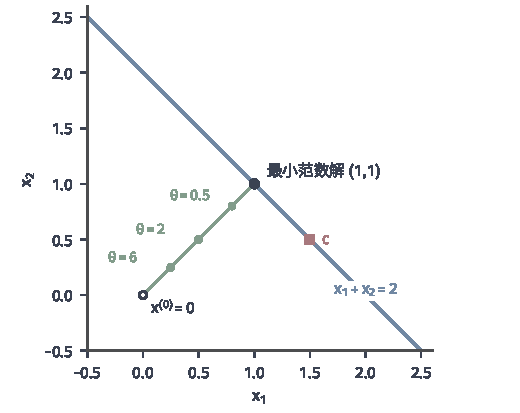
\includegraphics[width=88mm]{figures/03-optimization-evolution-and-signals/01-optimization/matplotlib/c7-inner-selection/figure.pdf}
  \caption{内层多解时的选解。蓝线是$\theta=0$时内层$\frac12(x_1+x_2-2)^2$的解集；绿线是$\theta>0$时的唯一解$\frac2{2+\theta}(1,1)$随$\theta$的轨迹，标出$\theta=0.5,2,6$三点。$\theta\to0^+$时它趋于最小范数解$(1,1)$，从原点出发的梯度下降也停在这里；外层目标点$\bm c=(1.5,0.5)$虽在解集上，只有乐观规则会选它。}
  \label{fig:opt-mmb-inner-selection}
\end{figure}

\paragraph{三种外层目标}
即使内层损失相同，实际计算中也会出现三个不同的外层目标。第一是理想的全局选解目标$J$，它要求内层被精确地全局求解。第二是局部分支目标$\widehat J$：内层非凸时，我们往往只能沿某个局部极小点随$\bm\theta$连续变化的分支计算，这一分支未必处处是全局最优解。第三是有限步目标$J_T(\bm\theta)=L_{\mathrm{out}}(\bm x^{(T)}(\bm\theta),\bm\theta)$，其中$\bm x^{(T)}(\bm\theta)$是内层算法从给定初值运行$T$步的输出。三者的最小点可以不同，导数也可以不同。上面的二维例子还说明，内层最优值相同不等于外层评价相同：直线$x_1+x_2=2$上每一点的内层损失都是零，外层值却从$0$到$+\infty$都有。外层目标对$\bm\theta$的梯度称为\term{超梯度}（hypergradient），下面两小节分别对$J_T$和$\widehat J$求超梯度，图~\ref{fig:opt-mmb-bilevel-chain}把两条计算路线并排画出。

\begin{figure*}[!htbp]
  \centering
  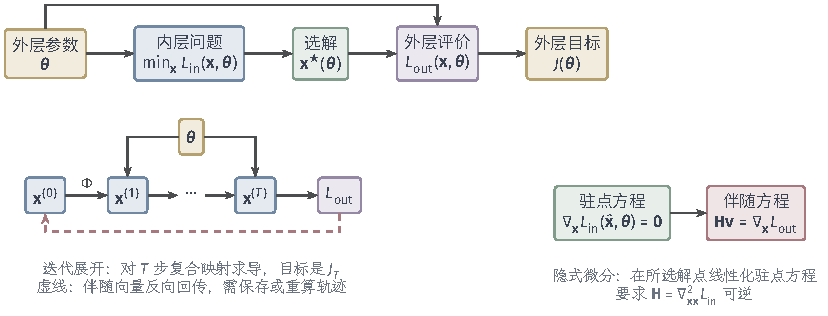
\includegraphics[width=140.1mm]{figures/03-optimization-evolution-and-signals/01-optimization/tikz/c7-bilevel-chain/figure.pdf}
  \caption{双层问题的复合结构与两种超梯度。上行：外层参数$\bm\theta$同时进入内层问题和外层评价，内层按选解规则给出$\bm x^\star(\bm\theta)$，外层目标$J$是两者的复合。左下：迭代展开把$T$步内层更新$\Phi$看成依赖$\bm\theta$的复合映射，虚线表示反向累计时伴随向量从外层评价逐步传回初值，需要保存或重算整条轨迹。右下：隐式微分只在所选解点处线性化驻点方程，解一个以内层Hessian为系数的伴随方程。}
  \label{fig:opt-mmb-bilevel-chain}
\end{figure*}

\subsection{迭代展开法}
\label{sec:opt-mmb-unrolling}

\paragraph{把有限步算法看成复合映射}
设内层用固定步长$\eta$的梯度下降，$L_{\mathrm{in}}$二阶连续可微：
\[
\bm x^{(t+1)}=\Phi(\bm x^{(t)},\bm\theta)=\bm x^{(t)}-\eta\nabla_{\bm x}L_{\mathrm{in}}(\bm x^{(t)},\bm\theta),\qquad t=0,\dots,T-1.
\]
$\bm x^{(T)}$是$\bm\theta$经过$T$层复合得到的函数，对它求导只需反复使用链式法则，这就是\term{迭代展开法}（unrolled differentiation）。记$\bm D^{(t)}=\partial\bm x^{(t)}/\partial\bm\theta\in\mathbb R^{d\times p}$，
\[
\bm A^{(t)}=\bm I-\eta\nabla^2_{\bm x\bm x}L_{\mathrm{in}}(\bm x^{(t)},\bm\theta),\qquad
\bm C^{(t)}=-\eta\nabla^2_{\bm x\bm\theta}L_{\mathrm{in}}(\bm x^{(t)},\bm\theta)\in\mathbb R^{d\times p}.
\]
对更新式两边关于$\bm\theta$求导，$\bm x^{(t)}$本身依赖$\bm\theta$，所以
\begin{equation}
\label{eq:opt-mmb-forward-sensitivity}
\begin{aligned}
\bm D^{(t+1)}&=\bm A^{(t)}\bm D^{(t)}+\bm C^{(t)},\\
\nabla J_T(\bm\theta)&=(\bm D^{(T)})^\top\nabla_{\bm x}L_{\mathrm{out}}(\bm x^{(T)},\bm\theta)+\nabla_{\bm\theta}L_{\mathrm{out}}(\bm x^{(T)},\bm\theta).
\end{aligned}
\end{equation}
初值$\bm D^{(0)}=\partial\bm x^{(0)}/\partial\bm\theta$通常为零，但若用上一个$\bm\theta$的解热启动，初值也依赖$\bm\theta$，这一项不能丢。这里用到的多元复合函数链式法则，以及下一小节要用的隐函数定理，都可参考\BookChapterRef{chap:multivariate-calculus}{卷一“多元函数微分”章}。

\paragraph{完整状态与其他参数}
若内层用带动量或自适应统计的方法，一步更新依赖的不只是$\bm x^{(t)}$。这时要把完整状态$\bm z^{(t)}$（例如参数与动量）作为展开对象，更新写成$\bm z^{(t+1)}=\Phi_t(\bm z^{(t)},\bm\theta)$，递推改为$\bm D_{\bm z}^{(t+1)}=\partial_{\bm z}\Phi_t\,\bm D_{\bm z}^{(t)}+\partial_{\bm\theta}\Phi_t$。只对$\bm x$部分求导会漏掉动量对$\bm\theta$的依赖。若步长、动量系数本身就是外层要调的参数，它们也出现在$\partial_{\bm\theta}\Phi_t$中。更新中含有截断、符号或取最大值等运算时，复合映射只在不切换分支的区域可微，求导前要确认迭代没有落在切换点上。

\paragraph{正则参数例中的展开}
在例~\eqref{eq:opt-mmb-ridge-bilevel}中取$x^{(0)}=0$、$\eta=\frac12$。这时$\nabla^2_{xx}L_{\mathrm{in}}=1+\theta$，$\nabla^2_{x\theta}L_{\mathrm{in}}=x$，所以$A^{(t)}=1-\frac{1+\theta}2$，$C^{(t)}=-\frac12x^{(t)}$。在$\theta=0$处$A^{(t)}=\frac12$，迭代与导数依次为
\[
x^{(0)},x^{(1)},x^{(2)},x^{(3)}=0,\ \tfrac32,\ \tfrac94,\ \tfrac{21}8;\qquad
D^{(0)},D^{(1)},D^{(2)},D^{(3)}=0,\ 0,\ -\tfrac34,\ -\tfrac32.
\]
于是$J_2'(0)=(x^{(2)}-1)D^{(2)}=-\frac{15}{16}$，$J_3'(0)=-\frac{39}{16}$；而理想目标的导数是$J'(0)=(x^\star-1)\frac{\mathrm dx^\star}{\mathrm d\theta}=2\times(-3)=-6$。三个数都是正确的导数，只是对应不同的目标。$J_1$尤其特别：从$x^{(0)}=0$出发，第一步的梯度$-(3-x^{(0)})+\theta x^{(0)}=-3$与$\theta$无关，于是$x^{(1)}=\frac32$对所有$\theta$都相同，$J_1$是常数，展开一步完全看不到正则的作用。

不同的$T$还会移动外层的最小点。$x^{(2)}=\frac94-\frac34\theta$，它在$\theta=\frac53$时等于验证观测$1$，所以$J_2$的最小点是$\frac53$，而$J$的最小点是$2$。图~\ref{fig:opt-mmb-unroll}左栏画出了$x^{(T)}(\theta)$与$x^\star(\theta)$：各曲线穿过水平线$x=1$的位置就是相应外层目标的最小点，曲线在$\theta=0$处的斜率就是$D^{(T)}$。本例中$|A^{(t)}|=\frac12<1$，导数$D^{(T)}$随$T$收敛到$\mathrm dx^\star/\mathrm d\theta$；一般问题中迭代点收敛并不自动推出导数收敛，后者还需要$\bm A^{(t)}$的谱半径一致地小于$1$一类的条件。还要注意固定步长$\eta=\frac12$只在$\theta<3$时使内层迭代收敛，$\theta\geq3$时$J_T$描述的是一个发散算法的输出。

\begin{figure*}[!htbp]
  \centering
  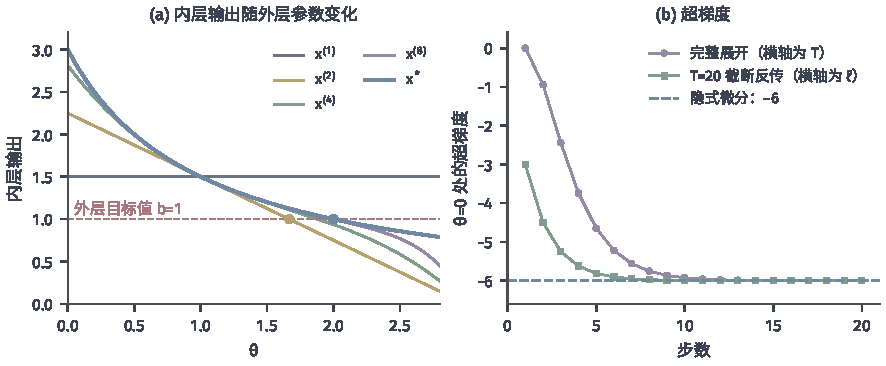
\includegraphics[width=150mm]{figures/03-optimization-evolution-and-signals/01-optimization/matplotlib/c7-unroll-vs-implicit/figure.pdf}
  \caption{正则参数例~\eqref{eq:opt-mmb-ridge-bilevel}的展开与隐式超梯度，内层梯度下降取$x^{(0)}=0$、$\eta=1/2$。(a)内层输出随$\theta$的变化：$x^{(T)}(\theta)$（$T=1,2,4,8$）与精确解$x^\star=3/(1+\theta)$；红虚线是验证观测$1$，曲线与它的交点是外层最小点，$J_2$在$\theta=5/3$、$J$在$\theta=2$；所有曲线在$\theta=1$相交，因为此时$A^{(t)}=0$，一步即得精确解。(b)$\theta=0$处的超梯度：紫线是完整展开的$J_T'(0)$随$T$的变化（$0,-15/16,-39/16,\dots$），绿线是$T=20$时只回传最后$\ell$步的截断结果，蓝虚线是隐式微分给出的$J'(0)=-6$。}
  \label{fig:opt-mmb-unroll}
\end{figure*}

\paragraph{前向灵敏度与反向累计}
递推~\eqref{eq:opt-mmb-forward-sensitivity}是前向计算：它随内层迭代同步更新$d\times p$矩阵$\bm D^{(t)}$，每步需要$\nabla^2_{\bm x\bm x}L_{\mathrm{in}}$与$p$个向量的乘积，存储$O(dp)$，不需要保存轨迹。外层参数很多时（例如每个样本一个权重），$p$与$d$同阶，这一代价不可接受。把$\nabla J_T$展开成乘积之和，可以从后往前累计：
\begin{equation}
\label{eq:opt-mmb-reverse}
\begin{aligned}
&\bm q^{(T)}=\nabla_{\bm x}L_{\mathrm{out}}(\bm x^{(T)},\bm\theta),\\
&\bm h\gets\bm h+(\bm C^{(t)})^\top\bm q^{(t+1)},\quad
\bm q^{(t)}=(\bm A^{(t)})^\top\bm q^{(t+1)},\qquad t=T-1,\dots,0,
\end{aligned}
\end{equation}
从$\bm h=\nabla_{\bm\theta}L_{\mathrm{out}}(\bm x^{(T)},\bm\theta)$开始，最后再加上初值项$(\bm D^{(0)})^\top\bm q^{(0)}$，得到的$\bm h$就是$\nabla J_T(\bm\theta)$。反向计算每步只需一次Hessian--向量积和一次混合二阶导数与向量的乘积，与$p$无关；代价是计算$\bm A^{(t)},\bm C^{(t)}$需要$\bm x^{(t)}$，必须保存整条轨迹，存储$O(Td)$。折中做法是每隔$k$步保存一个检查点，反向时从最近的检查点重算中间状态，存储约为$T/k+k$个状态，额外约一次前向计算；取$k\approx\sqrt T$时存储降到$O(\sqrt Td)$。

\paragraph{截短前向与截断反传}
为了省时，常见两种截断，它们的性质完全不同。一种是减少前向步数，用$J_{T'}$（$T'<T$）代替$J_T$：这改变了目标本身，上例中$J_2$与$J$的最小点已经相差$\frac13$。另一种是前向仍跑满$T$步，反向只回传最后$\ell$步：它近似的仍是$J_T$的导数。由$\bm D^{(T)}=\bm A^{(T-1)}\cdots\bm A^{(T-\ell)}\bm D^{(T-\ell)}+\sum_{t=T-\ell}^{T-1}\bm A^{(T-1)}\cdots\bm A^{(t+1)}\bm C^{(t)}$，被舍去的正是第一项，误差满足
\[
\lVert\text{截断误差}\rVert_2\leq\lVert\nabla_{\bm x}L_{\mathrm{out}}(\bm x^{(T)},\bm\theta)\rVert_2\,\lVert\bm A^{(T-1)}\cdots\bm A^{(T-\ell)}\rVert_2\,\lVert\bm D^{(T-\ell)}\rVert_2.
\]
内层是收缩迭代时，这一误差随$\ell$几何衰减。图~\ref{fig:opt-mmb-unroll}右栏中$A^{(t)}=\frac12$，只回传一步得到$-3$，回传约十步后已与完整展开几乎相同。

\subsection{隐式微分法}
\label{sec:opt-mmb-implicit}

迭代展开的存储和计算都随$T$增长，而且求出的是有限步目标的导数。若内层已经求解到某个非退化的局部极小点附近，可以绕过整条轨迹，直接对“梯度为零”这个方程求导。

\paragraph{选定分支上的导数}
设$\hat{\bm x}_0$是$L_{\mathrm{in}}(\cdot,\bm\theta_0)$的局部极小点，满足驻点方程$\nabla_{\bm x}L_{\mathrm{in}}(\hat{\bm x}_0,\bm\theta_0)=\bm 0$，且$L_{\mathrm{in}}$在$(\hat{\bm x}_0,\bm\theta_0)$附近二阶连续可微。把驻点方程看作关于$(\bm x,\bm\theta)$的$d$个方程，它对$\bm x$的Jacobian就是内层Hessian。

\begin{theorem}[解分支的可微性]
\label{thm:opt-mmb-implicit-branch}
若$\bm H_0=\nabla^2_{\bm x\bm x}L_{\mathrm{in}}(\hat{\bm x}_0,\bm\theta_0)$可逆，则存在$\bm\theta_0$的邻域$U$、$\hat{\bm x}_0$的邻域$V$和唯一的连续可微映射$\hat{\bm x}:U\to V$，使$\hat{\bm x}(\bm\theta_0)=\hat{\bm x}_0$且$\nabla_{\bm x}L_{\mathrm{in}}(\hat{\bm x}(\bm\theta),\bm\theta)=\bm 0$；其导数为
\begin{equation}
\label{eq:opt-mmb-implicit-derivative}
\frac{\partial\hat{\bm x}}{\partial\bm\theta}=-\bm H^{-1}\bm B,\qquad
\bm H=\nabla^2_{\bm x\bm x}L_{\mathrm{in}}(\hat{\bm x}(\bm\theta),\bm\theta),\quad
\bm B=\nabla^2_{\bm x\bm\theta}L_{\mathrm{in}}(\hat{\bm x}(\bm\theta),\bm\theta).
\end{equation}
若$\bm H_0\succ\bm 0$，则缩小$U$后，$\hat{\bm x}(\bm\theta)$都是严格局部极小点。
\end{theorem}

\begin{proof}
前半部分是卷一隐函数定理应用于方程$\nabla_{\bm x}L_{\mathrm{in}}(\bm x,\bm\theta)=\bm 0$的结论，该方程关于$\bm x$的Jacobian正是$\bm H$；对恒等式$\nabla_{\bm x}L_{\mathrm{in}}(\hat{\bm x}(\bm\theta),\bm\theta)=\bm 0$两边关于$\bm\theta$求导得$\bm H\,\partial\hat{\bm x}/\partial\bm\theta+\bm B=\bm 0$。Hessian连续而正定矩阵的最小特征值连续依赖矩阵，所以$\bm H_0\succ\bm 0$时在$\bm\theta_0$附近$\bm H\succ\bm 0$，再由第~\ref{chap:optimization}章的二阶充分条件，驻点$\hat{\bm x}(\bm\theta)$是严格局部极小点。
\end{proof}

把式~\eqref{eq:opt-mmb-implicit-derivative}代入外层链式法则，得到局部分支目标$\widehat J(\bm\theta)=L_{\mathrm{out}}(\hat{\bm x}(\bm\theta),\bm\theta)$的梯度，称为\term{隐式超梯度}（implicit hypergradient）：
\begin{equation}
\label{eq:opt-mmb-implicit-hypergradient}
\nabla\widehat J(\bm\theta)=\nabla_{\bm\theta}L_{\mathrm{out}}-\bm B^\top\bm v,\qquad
\bm H\bm v=\nabla_{\bm x}L_{\mathrm{out}},
\end{equation}
其中各导数都在$(\hat{\bm x}(\bm\theta),\bm\theta)$处取值，并用了$\bm H$的对称性。实际计算从不显式形成$\bm H^{-1}$，而是解伴随方程$\bm H\bm v=\nabla_{\bm x}L_{\mathrm{out}}$。$\bm H$正定时可用共轭梯度法，每次迭代只需一次Hessian--向量积，迭代线性求解器的做法见\BookChapterRef{chap:linear-equations-and-optimization}{卷一“线性方程与矩阵方程”章}。整个计算如算法~\ref{alg:opt-mmb-implicit}所示，它只用到解点处的信息，存储为$O(d)$，与内层跑了多少步无关。

\begin{algorithm}[隐式超梯度]
\label{alg:opt-mmb-implicit}
\begin{algorithmic}[1]
\Require 外层参数$\bm\theta$，内层求解器与容差$\varepsilon_{\mathrm{in}}$，伴随求解容差$\varepsilon_{\mathrm{lin}}$
\Ensure 近似超梯度$\tilde{\bm h}$，内层残差$\bm r_{\mathrm{in}}$与伴随残差$\bm r_{\mathrm{lin}}$
\State 求解内层到$\tilde{\bm x}$，使$\bm r_{\mathrm{in}}=\nabla_{\bm x}L_{\mathrm{in}}(\tilde{\bm x},\bm\theta)$满足$\lVert\bm r_{\mathrm{in}}\rVert_2\leq\varepsilon_{\mathrm{in}}$
\State 检查$\tilde{\bm x}$处Hessian的最小特征值（或其可靠下界）为正，否则报告分支退化
\State 用共轭梯度法近似求解$\bm H(\tilde{\bm x})\bm v=\nabla_{\bm x}L_{\mathrm{out}}(\tilde{\bm x},\bm\theta)$，得$\tilde{\bm v}$及残差$\bm r_{\mathrm{lin}}$，直到$\lVert\bm r_{\mathrm{lin}}\rVert_2\leq\varepsilon_{\mathrm{lin}}$
\State $\tilde{\bm h}\gets\nabla_{\bm\theta}L_{\mathrm{out}}(\tilde{\bm x},\bm\theta)-\bm B(\tilde{\bm x})^\top\tilde{\bm v}$
\end{algorithmic}
\end{algorithm}

在正则参数例中，$H=1+\theta$，$B=x$，伴随方程给出$v=(x-1)/(1+\theta)$，于是$\widehat J'(\theta)=-x(x-1)/(1+\theta)$。$\theta=0$、$x=3$时得$-6$，与直接对$J$求导一致，也是图~\ref{fig:opt-mmb-unroll}右栏中展开导数随$T$趋近的值。

定理~\ref{thm:opt-mmb-implicit-branch}只说明一个局部分支是可微的，并不说明这个分支就是规定的选解。内层非凸时，沿分支算出的是$\widehat J$的导数；只有当该分支在所考虑的$\bm\theta$范围内始终是全局最小点（或始终符合规定的选解规则）时，才有$\widehat J=J$。第~\ref{sec:opt-mmb-outer}小节会给出两者分离的具体例子。

\paragraph{两类残差及其放大}
算法~\ref{alg:opt-mmb-implicit}有两处近似：内层点$\tilde{\bm x}$不是精确驻点，伴随方程也只解到残差$\bm r_{\mathrm{lin}}=\bm H(\tilde{\bm x})\tilde{\bm v}-\nabla_{\bm x}L_{\mathrm{out}}(\tilde{\bm x},\bm\theta)$。为了分别追踪它们，把式~\eqref{eq:opt-mmb-implicit-hypergradient}的右端看作内层点的函数
\[
\bm h(\bm x)=\nabla_{\bm\theta}L_{\mathrm{out}}(\bm x,\bm\theta)-\bm B(\bm x)^\top\bm H(\bm x)^{-1}\nabla_{\bm x}L_{\mathrm{out}}(\bm x,\bm\theta),
\]
真值是$\bm h(\hat{\bm x})$。

\begin{lemma}[超梯度的误差分解]
\label{lem:opt-mmb-hypergradient-error}
设$N$是含$\hat{\bm x}$与$\tilde{\bm x}$的凸集，在$N$上$\nabla^2_{\bm x\bm x}L_{\mathrm{in}}(\cdot,\bm\theta)\succeq\mu\bm I$（$\mu>0$），且$\bm h$在$N$上是$K_h$-Lipschitz的。则
\[
\lVert\tilde{\bm h}-\bm h(\hat{\bm x})\rVert_2\leq\frac{K_h}{\mu}\lVert\bm r_{\mathrm{in}}\rVert_2+\frac{\lVert\bm B(\tilde{\bm x})\rVert_2}{\mu}\lVert\bm r_{\mathrm{lin}}\rVert_2.
\]
\end{lemma}

\begin{proof}
把误差拆成$\tilde{\bm h}-\bm h(\tilde{\bm x})$与$\bm h(\tilde{\bm x})-\bm h(\hat{\bm x})$。前者等于$-\bm B(\tilde{\bm x})^\top\bigl(\tilde{\bm v}-\bm H(\tilde{\bm x})^{-1}\nabla_{\bm x}L_{\mathrm{out}}\bigr)=-\bm B(\tilde{\bm x})^\top\bm H(\tilde{\bm x})^{-1}\bm r_{\mathrm{lin}}$，而$\lVert\bm H(\tilde{\bm x})^{-1}\rVert_2\leq1/\mu$。后者不超过$K_h\lVert\tilde{\bm x}-\hat{\bm x}\rVert_2$。最后，沿$N$中连接两点的线段积分Hessian得$\langle\nabla_{\bm x}L_{\mathrm{in}}(\tilde{\bm x})-\nabla_{\bm x}L_{\mathrm{in}}(\hat{\bm x}),\tilde{\bm x}-\hat{\bm x}\rangle\geq\mu\lVert\tilde{\bm x}-\hat{\bm x}\rVert_2^2$，左侧第二个梯度为零，由Cauchy--Schwarz不等式得$\lVert\tilde{\bm x}-\hat{\bm x}\rVert_2\leq\lVert\bm r_{\mathrm{in}}\rVert_2/\mu$。
\end{proof}

两项分别来自“在错误的点上求导”与“在正确的点上没解准伴随方程”，各自需要单独控制，压低其中一项并不能控制另一项。小曲率$\mu$同时放大两者，而且$K_h$本身通常也含有$1/\mu$。看一个可以直接算的例子：$L_{\mathrm{in}}(x,\theta)=\frac\mu2x^2-\theta x$，$L_{\mathrm{out}}=\frac12(x-1)^2$。这时$\hat x=\theta/\mu$，$H=\mu$，$B=-1$，$h(x)=(x-1)/\mu$。内层残差$r_{\mathrm{in}}=\mu\tilde x-\theta$造成点误差$r_{\mathrm{in}}/\mu$，再经$h$放大为$r_{\mathrm{in}}/\mu^2$；伴随残差造成$v$的误差$r_{\mathrm{lin}}/\mu$，超梯度误差也是$r_{\mathrm{lin}}/\mu$。取$\mu=0.01$、两个残差都是$10^{-4}$，前者使超梯度偏差$1$，后者偏差$0.01$。内层“几乎平坦”时，看似很小的残差也会让超梯度失去意义。

\paragraph{公式的适用边界}
式~\eqref{eq:opt-mmb-implicit-hypergradient}依赖三件事：内层无约束、解点处梯度为零、Hessian可逆。内层带约束且解在边界上时，驻点方程要换成KKT系统；活动约束集合保持不变时，可以对KKT方程组整体应用同样的隐函数论证，第~\ref{chap:constrained-optimization}章讨论了这种参数敏感性，而活动集切换的参数处解映射一般不可微。Hessian奇异时（例如两条分支在折点处合并），定理~\ref{thm:opt-mmb-implicit-branch}的条件不成立，导数可能趋于无穷。这些情形都不能直接套用无约束内点公式。

\subsection{外层求解与结果核验}
\label{sec:opt-mmb-outer}

有了超梯度，外层就是一个以$J_T$或$\widehat J$为目标的普通优化问题：$\Theta=\mathbb R^p$时用第~\ref{chap:opt-smooth}章的梯度法，$\Theta$是闭凸集时用第~\ref{chap:opt-nonsmooth}章的投影梯度法，超梯度由小批量数据估计时用第~\ref{chap:opt-stochastic-block}章的随机方法。与普通问题不同的是，每次得到的方向都带有内层与伴随求解的误差，求解前要先确定这些误差允许有多大。

\paragraph{近似超梯度下的外层进展}
设外层目标$J$（指$J_T$或$\widehat J$中选定的一个）在$\mathbb R^p$上是$L_J$-光滑的，下有界，下确界为$J_{\inf}$。外层迭代$\bm\theta^{(k+1)}=\bm\theta^{(k)}-\eta\tilde{\bm h}^{(k)}$，其中$\tilde{\bm h}^{(k)}=\nabla J(\bm\theta^{(k)})+\bm e^{(k)}$。

\begin{lemma}[近似超梯度的下降]
\label{lem:opt-mmb-inexact-outer}
取$\eta=1/L_J$，则$J(\bm\theta^{(k+1)})\leq J(\bm\theta^{(k)})-\frac\eta2\lVert\nabla J(\bm\theta^{(k)})\rVert_2^2+\frac\eta2\lVert\bm e^{(k)}\rVert_2^2$，因而
\[
\min_{0\leq k<K}\lVert\nabla J(\bm\theta^{(k)})\rVert_2^2\leq\frac{2L_J\bigl(J(\bm\theta^{(0)})-J_{\inf}\bigr)}K+\max_{0\leq k<K}\lVert\bm e^{(k)}\rVert_2^2.
\]
\end{lemma}

\begin{proof}
记$\bm g=\nabla J(\bm\theta^{(k)})$，$\bm e=\bm e^{(k)}$。由第~\ref{chap:opt-smooth}章的二次上界，
\[
J(\bm\theta^{(k+1)})\leq J(\bm\theta^{(k)})-\eta\langle\bm g,\bm g+\bm e\rangle+\frac{L_J\eta^2}2\lVert\bm g+\bm e\rVert_2^2.
\]
代入$L_J\eta=1$并展开$\lVert\bm g+\bm e\rVert_2^2$，交叉项$\langle\bm g,\bm e\rangle$恰好抵消，得到第一式。对$k=0,\dots,K-1$求和，用$J(\bm\theta^{(K)})\geq J_{\inf}$并以最小值代替平均值即得第二式。
\end{proof}

引理说明，超梯度误差的大小直接决定外层能达到的驻点精度：若要求$\lVert\nabla J\rVert_2\leq\varepsilon$，误差至少要控制在$\varepsilon$量级，再由引理~\ref{lem:opt-mmb-hypergradient-error}换算成内层与伴随残差的容差。外层的光滑常数$L_J$本身由内外两层的性质共同决定，常常未知，这时用回溯步长，但要记住每次试探都要重新求解内层。

\paragraph{外层最小点的存在}
外层能否达到最小值，是一个与内层能否求解分开的问题。若$\Theta$非空紧且$J$连续，由第~\ref{chap:optimization}章的存在性结论，外层最小点存在。内层唯一解保证$J$有定义，再加上下面的连续性条件才保证$J$连续。设对每个$\bm\theta$，$L_{\mathrm{in}}(\cdot,\bm\theta)$可微且$\mu$-强凸（$\mu$与$\bm\theta$无关），对每个固定的$\bm x$，$\nabla_{\bm x}L_{\mathrm{in}}(\bm x,\cdot)$连续。记$\bm a=\bm x^\star(\bm\theta)$，$\bm b=\bm x^\star(\bm\theta')$，由强凸函数梯度的强单调性与$\nabla_{\bm x}L_{\mathrm{in}}(\bm a,\bm\theta)=\bm 0$，
\[
\begin{aligned}
\mu\lVert\bm a-\bm b\rVert_2^2&\leq\langle\nabla_{\bm x}L_{\mathrm{in}}(\bm a,\bm\theta)-\nabla_{\bm x}L_{\mathrm{in}}(\bm b,\bm\theta),\bm a-\bm b\rangle\\
&\leq\lVert\nabla_{\bm x}L_{\mathrm{in}}(\bm b,\bm\theta)-\nabla_{\bm x}L_{\mathrm{in}}(\bm b,\bm\theta')\rVert_2\,\lVert\bm a-\bm b\rVert_2,
\end{aligned}
\]
其中最后一步用了$\nabla_{\bm x}L_{\mathrm{in}}(\bm b,\bm\theta')=\bm 0$。令$\bm\theta\to\bm\theta'$，右侧趋于零，所以$\bm x^\star$连续；$L_{\mathrm{out}}$连续时$J$也连续。这正是第~\ref{chap:opt-smooth}章强凸目标扰动界的思路。

内层不唯一时，即使$\Theta$紧，外层最小值也可能达不到。取倾斜的双势阱
\begin{equation}
\label{eq:opt-mmb-tilted-well}
L_{\mathrm{in}}(x,\theta)=\tfrac14x^4-\tfrac12x^2+\theta x,\qquad L_{\mathrm{out}}(x)=\tfrac12(x-1)^2,\qquad\Theta=[-\tfrac14,\tfrac14].
\end{equation}
驻点满足$x^3-x+\theta=0$，在$|\theta|<2/(3\sqrt3)\approx0.385$时有左右两个局部极小点。比较两个阱底的值，$\theta<0$时右阱更低，$\theta>0$时左阱更低，$\theta=0$时两者并列于$x=\pm1$。于是全局选解在$\theta<0$时取右分支（其上$x>1$，$J>0$且$\theta\to0^-$时$J\to0$），在$\theta>0$时取左分支（$x<-1$，$J>2$）。在$\theta=0$处，乐观规则选$x=1$，$J(0)=0$，最小值达到；悲观规则选$x=-1$，$J(0)=2$，此时$\inf_\Theta J=0$却没有任何$\theta$达到它。

\paragraph{分支核验}
图~\ref{fig:opt-mmb-branch-switch}画出了这个例子的两条分支。沿右分支，定理~\ref{thm:opt-mmb-implicit-branch}给出$\mathrm dx/\mathrm d\theta=-1/(3x^2-1)$，在$\theta=0$处为$-\frac12$，右分支目标$\widehat J$在$\theta=0$的导数是$(x-1)\cdot(-\frac12)=0$，看上去$\theta=0$是一个平稳的外层驻点。但这个公式只描述右分支：$\theta$一旦越过零，全局选解跳到左分支，真正的$J$跳到$2$以上。右分支一直延续到折点$\theta=2/(3\sqrt3)$，那里$3x^2-1=0$，Hessian奇异，分支终止。若外层迭代从$\theta<0$出发并用热启动沿右分支跟踪，它会把右分支误当作全局选解，越过零以后仍然报告很小的$J$。

\begin{figure*}[!htbp]
  \centering
  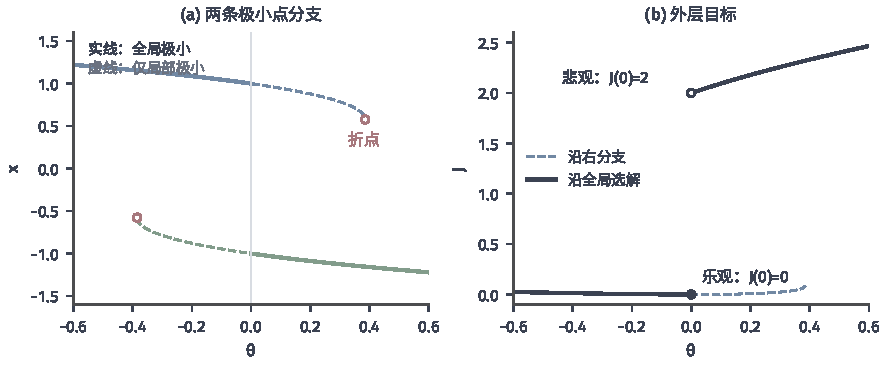
\includegraphics[width=150mm]{figures/03-optimization-evolution-and-signals/01-optimization/matplotlib/c7-branch-switch/figure.pdf}
  \caption{倾斜双势阱~\eqref{eq:opt-mmb-tilted-well}的内层分支与外层目标。(a)驻点方程$x^3-x+\theta=0$的两条局部极小点分支（右分支蓝、左分支绿）；实线段是全局极小点，虚线段只是局部极小点；空心圆是折点$\theta=\pm2/(3\sqrt3)$，此处Hessian$3x^2-1$为零。(b)外层值$\frac12(x-1)^2$：黑色实线沿全局选解，在$\theta=0$处跳变；蓝色虚线沿右分支，光滑地经过$\theta=0$。$\theta=0$处乐观规则取实心点$0$，悲观规则取空心点$2$。}
  \label{fig:opt-mmb-branch-switch}
\end{figure*}

因此，改变外层参数时，需要随时核验内层选解是否仍在同一可微分支，并且这条分支是否仍符合规定的选解规则。可行的做法包括：监测内层Hessian的最小特征值，接近零时警惕折点；在若干个$\bm\theta$处从不同初值重新求解内层，比较各局部解的内层值；分支切换时，不再使用跨越切换点的同一个隐式公式。报告结果时应同时给出所用的选解规则与分支、外层值，以及由引理~\ref{lem:opt-mmb-hypergradient-error}估计的超梯度误差。提高内层与伴随求解的精度，只能减小同一个目标上的数值误差；若把局部分支误当作全局选解，这是目标定义上的错误，再精确的计算也不能消除。

\section{三类问题的求解结果与成本}
\label{sec:opt-mmb-results-costs}

前三节分别处理了三类问题，用到的工具有很多重叠：梯度、投影、乘子、二次上界。工具相同容易让人以为它们的结果也可以用同一把尺子衡量，例如把“共同下降方向的范数小于$10^{-6}$”“外梯度残差小于$10^{-6}$”“超梯度小于$10^{-6}$”都称为“已收敛”。本节以“得到并检验一个规定的答案”为共同任务，先核对三类输出各自满足什么关系，再核对为得到它付出了什么。三类问题的残差数值含义不同，不作相互排序。

\subsection{不同最优性标准}
\label{sec:opt-mmb-standards}

\paragraph{各自改变了标量优化的哪一项}
标量优化由三部分组成：候选集合、比较候选的规则、以及计算目标值的方式。多目标问题保留了候选集合和目标的计算方式，改变的是比较规则：向量之间只有支配这一偏序，答案因而是一个集合，选出其中一点需要额外的偏好。极小极大问题保留了数值比较，改变的是目标值的计算方式：$\bar\phi(\bm x)$本身是一个优化问题的最优值，而且依赖于双方的选择次序。双层问题同样改变目标值的计算方式，但内层有自己的目标，外层值依赖于内层解如何选出；选解规则不同，外层目标就是不同的函数。三类问题都会用到梯度和乘子，这并不让它们共享一个解概念。

\paragraph{局部判据、全局证书与内层精度}
表~\ref{tab:opt-mmb-standards}逐项列出三类问题的局部判据能说明什么、有没有可以计算的全局证书，以及判据对内层计算的精度要求。

\begin{table*}[!htbp]
  \centering
  \small
  \begin{tabularx}{\linewidth}{@{}p{12mm}XXXX@{}}
    \toprule
    问题 & 局部判据 & 判据能支持的结论 & 可计算的全局证书 & 对内层精度的要求 \\
    \midrule
    多目标 & 梯度凸包的最小范数$\lVert\bar{\bm g}\rVert_2$ & 不存在一阶共同下降方向；各指标凸时为某个加权和的最小点，正权时为Pareto最优 & 凸情形下加权和的最优性证书；有限候选可逐一比较；阈值问题可用第~\ref{chap:constrained-optimization}章的对偶界 & 无内层；回溯须对每个指标检查 \\
    极小极大 & 投影残差$\lVert\bm u-\Pi_K(\bm u-\eta\bm F(\bm u))\rVert_2/\eta$ & 凸凹且可微时残差为零等价于鞍点；非凸时只说明是驻点 & 间隙$\bar\phi(\bm x)-\underline\phi(\bm y)$，须求两侧最优响应或其界 & 内层最大化不精确时只得到$\bar\phi$的下界 \\
    双层 & 超梯度范数$\lVert\nabla J_T\rVert_2$或$\lVert\nabla\widehat J\rVert_2$ & 对所选目标（有限步或局部分支）的一阶驻点 & 一般没有；还须另行核验选解规则与分支 & 内层残差与伴随残差共同决定超梯度误差，并被小曲率放大 \\
    \bottomrule
  \end{tabularx}
  \caption{三类问题的最优性标准。各行的判据针对不同对象，同样小的数值代表不同强度的结论。}
  \label{tab:opt-mmb-standards}
\end{table*}

表中第二、三列的差距是本章反复出现的主题。共同下降法停在$\bar{\bm g}=\bm 0$，可能是一个被支配的点（第~\ref{sec:opt-mmb-common-descent}小节的$f_1=f_2=-x^2$）；极小极大的零梯度点可能有正的间隙（$\phi=y^2-x^2$在原点的间隙为$2$）；双层问题的超梯度为零，可能只是局部分支上的驻点，而真正的选解在那里跳变（倾斜双势阱在$\theta=0$处）。因此报告结果时，应写明“满足了哪一个判据、对哪一个目标、在什么条件下它意味着什么”，而不是只写一个“已收敛”。

\subsection{同一输出要求下的计算代价}
\label{sec:opt-mmb-costs}

\paragraph{一轮外层迭代包含什么}
三类方法的一轮迭代，实际工作量差别很大。表~\ref{tab:opt-mmb-costs}以梯度、Hessian--向量积和投影为单位记录每轮代价，其中$m$是指标个数，$T$是内层步数，$k$是伴随方程的共轭梯度迭代次数。

\begin{table*}[!htbp]
  \centering
  \small
  \begin{tabularx}{\linewidth}{@{}p{30mm}XX@{}}
    \toprule
    方法 & 每轮主要计算 & 额外存储或开销 \\
    \midrule
    加权和、阈值约束 & 一个标量或约束优化问题的完整求解（每个权重或阈值一次） & 描出前沿需对许多权重或阈值重复求解 \\
    共同下降法 & $m$个梯度；$m$维单纯形二次规划（形成Gram矩阵需$O(m^2d)$）；每次回溯试探求$m$个指标值 & 存储$m$个梯度 \\
    同时梯度下降—上升 & 一组偏梯度，$X$、$Y$上各一次投影 & 报告间隙需另解两个最优响应问题 \\
    外梯度法 & 两组偏梯度，$X$、$Y$上各两次投影 & 同上；平均保证需累计试探点 \\
    迭代展开（反向） & $T$步内层更新；反向$T$次Hessian--向量积与混合导数乘积 & 存储$O(Td)$，或用检查点以重算换存储 \\
    迭代展开（前向） & $T$步内层更新，每步$p$次Hessian--向量积 & 存储$O(dp)$ \\
    隐式微分 & 内层求解到容差；约$k$次Hessian--向量积解伴随方程；一次混合导数乘积 & 存储$O(d)$；须检查Hessian正定 \\
    \bottomrule
  \end{tabularx}
  \caption{各方法一轮迭代的主要代价。双层方法的每一轮外层更新都包含一次完整的内层求解或展开。}
  \label{tab:opt-mmb-costs}
\end{table*}

“一轮外层更新”在这些方法中代表的工作量并不相同。外梯度一轮相当于两轮同时梯度下降—上升；双层方法的一轮外层更新，包含了一次内层优化（$T$步或求解到容差）再加上一次反向或伴随计算，可能是外层梯度步本身代价的成百上千倍。按轮数比较不同方法没有意义。

\paragraph{先固定输出要求，再比较路线}
比较求解路线之前，先固定要返回的东西及其容差：是只要可行性，还是要某个局部残差小于$\varepsilon$，还是要一个全局证书（例如间隙不超过$\varepsilon$）。然后在同一问题、同一要求下比较总代价。近似的内层计算必须按它对最终输出的影响计费：若内层只解到使超梯度误差为$\delta$的精度，那么由引理~\ref{lem:opt-mmb-inexact-outer}，外层最多只能把驻点残差压到$\delta$量级，再多的外层迭代都是浪费；反之，为了一个只需粗略方向的早期外层步把内层解到机器精度，同样是浪费。极小极大问题中，若最终要报告间隙，求两侧最优响应的代价可能与求解本身相当，也必须算入。

本章的三类问题都是静态的：比较、响应和嵌套都发生在一次决策之内。若决策随时间展开，后一步的选择依赖于前一步观察到的结果；若对象在反馈下运行，控制量又会改变后续状态；若多方同时行动且各有信息，最优响应要换成均衡概念。这些结构在卷五中依次加入，那里的博弈部分会在本章极小极大与最优响应的基础上研究多方响应及其演化，可参考\BookChapterRef{chap:game-theory-and-multi-agent-decision}{卷五“多方策略的响应与演化”章}。

\section{本章小结}
\label{sec:opt-mmb-summary}

章首提出的问题是：当候选的好坏不再由一个数直接决定时，“最优答案”是什么，怎样算出它，又怎样检查它。本章对三种结构分别作了回答。

多个指标共存时，支配关系先排除全面劣势的候选，剩下的Pareto集合通常不止一点。非空紧可行域与连续指标保证正权加权和有最小点，从而保证Pareto点存在。加权和用价格表达偏好，只能到达可达集合左下凸包上的点，凹陷中的Pareto点永远选不到，权重变化时解还可能跳变；阈值约束用上限表达偏好，能到达每个Pareto点，但不唯一的解只保弱Pareto性。不预设偏好时，梯度凸包中的最小范数元给出共同下降方向，它为零只说明一阶意义下不能同时改善，凸性与正权才把它加强为Pareto最优。

两组变量方向相反时，先规定次序：外层最小化的是对手最优响应构成的上包络，内层近似求解只给出它的下界。鞍点表示双方互为全局最优响应，间隙为零是它的可计算证书；紧凸凹条件保证上下值相等且鞍点存在，但不保证任何特定算法能找到它。双线性例中，同时梯度下降—上升向外螺旋，加上投影后循环，交替版本有界打转；外梯度法先试探、再从旧点校正，在凸凹且Lipschitz的条件下平均点的间隙以$O(1/T)$下降。

一个问题嵌套另一个问题的解时，先规定内层怎样选解：唯一解、乐观或悲观规则、指定算法的输出，各自给出不同的外层目标。迭代展开对有限步目标$J_T$精确求导，代价是保存或重算轨迹；隐式微分对局部分支目标$\widehat J$求导，只需解点处的伴随方程，但要求Hessian可逆，误差同时来自内层残差与伴随残差，小曲率会放大二者。展开与隐式两种导数在正则参数例中分别为$-15/16$与$-6$，二者都正确，差别在于目标不同。外层求解可以直接调用前面章节的光滑、投影和随机方法，但超梯度误差限定了外层能达到的精度，而把局部分支误当作全局选解的错误，任何计算精度都无法弥补。

三类问题共同提醒我们分开陈述四件事：答案是否存在，局部判据是否满足，算法是否在进展，以及有没有可以核对的全局证书。前面各章的标量方法在这里分别承担了一部分工作：加权和与阈值问题直接交给光滑与约束方法求解，投影与单调性支撑了外梯度的分析，二次上界与隐函数定理支撑了超梯度的计算与外层下降。下一章转向另一种扩展：未知量从有限维参数变成由数据决定的函数，双层结构也会在正则参数的选择中再次出现。

